\documentclass[a4paper, 11pt, oneside]{article} 

\usepackage[utf8]{inputenc} % Required for inputting international characters
\usepackage[T1]{fontenc} % Output font encoding for international characters

% Custom titling format

\usepackage{secdot}
\usepackage{titling}
\usepackage[margin=1.5in]{geometry}
\date{\today}



% Remove numbering from sections but keep them in TOC

\makeatletter
\def\@seccntformat#1{%
  \expandafter\ifx\csname c@#1\endcsname\c@section\else
  \csname the#1\endcsname\quad
  \fi}
\makeatother

\usepackage{amssymb}
\usepackage{amsmath}
\usepackage{graphicx}
\usepackage{animate}
\usepackage{floatrow}
\usepackage{caption}
\usepackage{booktabs}

% Importing graphics

\usepackage{svg}
\usepackage{siunitx}
\usepackage{tikz} 
\usepackage{pgfplots}

% Allows to place the legend below plot

\pgfplotsset{compat=newest} 

% Allows to enter the units nicely

\usepgfplotslibrary{units} 

% Cute boxes

\usepackage{xcolor}
\usepackage[framemethod=default]{mdframed}

\newmdenv[skipabove=7pt,
          skipbelow=7pt,
          rightline=false,
          leftline=true,
          topline=false,
          bottomline=false,
          linecolor=orange!60!gray,
          backgroundcolor=gray!15,
          innerleftmargin=5pt,
          innerrightmargin=2pt,
          innertopmargin=5pt,
          leftmargin=0cm,
          rightmargin=0cm,
          linewidth=3pt,
          innerbottommargin=5pt]{cBox}
      
      
% Setting for writing code
      
\usepackage{minted}
\usepackage{algorithm}
\usepackage{algorithmic}
\usepackage{beramono}

\newenvironment{code}[2][]
 {\VerbatimEnvironment
  \begin{minted}[
        frame=lines,
        framesep=2mm,
        baselinestretch=1.2,
        bgcolor=bg,
        linenos,
        fontsize=\footnotesize
        ]{#2}}
 {\end{minted}}
 

%% Defines background colour of code
\definecolor{bg}{rgb}{0.95, 0.95, 0.95}
 
%% Adds the º symbol
\usepackage{gensymb}

% Includes "References" in the table of contents

\usepackage[nottoc]{tocbibind}

\usepackage[autostyle = true]{csquotes}

\usepackage[backend=biber,style=ieee]{biblatex}
\urlstyle{same}
\addbibresource{bibliography.bib}

%% Allows subsubsubsections
 
\makeatletter
\renewcommand{\paragraph}{\@startsection{paragraph}{4}{0ex}%
    {-3.25ex plus -1ex minus -0.2ex}%
    {1.5ex plus 0.2ex}%
    {\normalfont\normalsize\bfseries}}
\makeatother
 
\stepcounter{secnumdepth}
\stepcounter{tocdepth}

% Hyperlinks settings

\usepackage{hyperref}

\hypersetup{
    colorlinks=false,
    linkcolor=blue,
    filecolor=magenta,      
    urlcolor=cyan,
}


%----------------------------------------------------------------------------------------
%	DOCUMENT
%----------------------------------------------------------------------------------------

\begin{document} 

% ANIMATION ON = 1 / ANIMATION OFF = 0
\newcounter{ANIMATION}
\setcounter{ANIMATION}{1}

% Includes the title page
\begin{titlepage} % Suppresses headers and footers on the title page

    \fontfamily{stix}\selectfont
	\centering % Centre everything on the title page
	\scshape % Use small caps for all text on the title page
	\vspace*{\baselineskip} % White space at the top of the page
	
%------------------------------------------------------------------------------------------------
%	                                    Title
%------------------------------------------------------------------------------------------------
	\vspace{5\baselineskip}
	
	\rule{\textwidth}{1.6pt}\vspace*{-\baselineskip}\vspace*{2pt} % Thick horizontal rule
	\rule{\textwidth}{0.4pt} % Thin horizontal rule
	
	\vspace{0.75\baselineskip} % Whitespace above the title
	
	{\LARGE DIGITAL ELECTRONICS NOTEBOOK\\} % Title
	
	\vspace{0.75\baselineskip} % Whitespace below the title
	
	\rule{\textwidth}{0.4pt}\vspace*{-\baselineskip}\vspace{3.2pt} % Thin horizontal rule
	\rule{\textwidth}{1.6pt} % Thick horizontal rule
	
	\vspace{1.5\baselineskip} % Whitespace after the title block


	%------------------------------------------------
	%	Editor(s)
	%------------------------------------------------
	
	{\scshape\Large Alejandro López Rodríguez \\} % Editor list
	
	\vspace{1.5\baselineskip} % Whitespace below the editor list
	
	\textit{Universidad Politécnica de Valencia\\ ETSID\\} 
	
	\vspace{2\baselineskip} % Whitespace after the title block
	\thedate
	
	\vfill % Whitespace between editor names and publisher logo

\end{titlepage}

% Table of contents

\thispagestyle{empty}
\setcounter{page}{0}
\tableofcontents
\clearpage

% Add later

% \listoffigures
% \listoftables
% \clearpage

% Document

\part{Programmable Logic Devices} 

\clearpage

\section{Laboratory Lecture 1: VHDL}

In this lab lecture we will design a logic circuit that will act as an interface between the output of an ADC, a 4-bit value, and an array of LEDs so as to represent said value in a visual manner.\medskip

To better understand the circuit that we will be working with, we will start by drawing a simple diagram:\medskip

\begin{figure}[H]
    \centering
    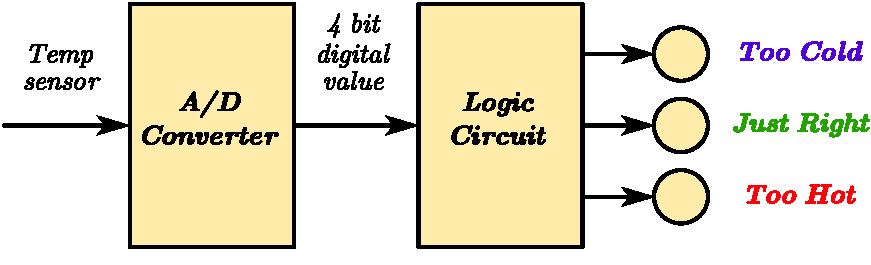
\includegraphics[width=\linewidth]{Graphics/Practice 1/Temp_ADC_Logic.pdf}
    \caption{Circuit block representation.}
    \label{fig:tempcircuit}
\end{figure}

As we can see in the diagram, there is a temperature sensor which output is fed into an analog-to-digital converter. The latter outputs a 4 bit digital value which serves as input to the logic circuit that we have to design. This circuit will interpret the  data and, based on it, it will turn on a specific LED to indicate the temperature range that the sensor is measuring, being these states the ones indicated in the diagram\medskip

To aid the design process, a table containing the possible output values of the ADC and their corresponding meaning is given:

\begin{table}[ht]
    \centering
        \begin{tabular}[t]{lcc}
            \toprule
            &\textbf{Digital Values}&\textbf{Category}\\
            \midrule
            &0000-1000&Too cold\\
            &1001-1010&Just right\\
            &1011-1111&Too hot\\
            \bottomrule
        \end{tabular}
        \caption{Possible states.}
\end{table}

Our job will consist in programming the logic circuit in order to obtain the desired behaviour. In this practice, as well as in the rest of the subject, we will make use of the GAL22V10. This IC, commonly found in the DIP package, though old, is still a very good choice for beginners, due to its simplicity and ease of use.\medskip

\newpage

To program the circuit, we will use the proprietary software designed for it, IspLever Classic. This program will allow us to synthesize and implement our VHDL code into the GAL SPLD. The main advantage of PLDs and FPGAs is the ability to program, using code, the HARDWARE part of our circuit, allowing us to obtain higher switching speeds and a faster response compared to what we would obtain if we were to use a microcontroller.\medskip

Writing some pseudocode before programming our circuit will surely come in handy later, as it is a nice way of organising the code and its different parts.

For this simple case, we came up with the following:\medskip

\begin{algorithm}
        \begin{algorithmic}
            \IF{digital value $\leq 8$}
            \STATE light only the \textcolor{blue}{Too Cold} indicator.
            \ELSIF{8 < digital value < 11}
            \STATE light only the \textcolor{green}{Just Right} indicator.
            \ELSE{}
            \STATE light only the \textcolor{red}{Too Hot} indicator.
            \ENDIF
        \end{algorithmic}
\end{algorithm}

Before starting programming our circuit, we will first define the basic parts of any VHDL program:

\subsection{Library}

One of the most important parts of any VHDL program is the inclusion of several, important libraries.\textbf{Libraries} are pre-written chunks of code that allow us to focus on the development of our code without having to worry too much about the technical and laborious parts of the language itself.

The structure of this part is as follows:

\begin{code}{vhdl}
library ieee;
use ieee.std_logic_1164.all;
use ieee.std_logic_arith.all;
use ieee.std_logic_unsigned.all;
\end{code}

Here we can find a library clause, for instance, \textbf{library ieee;} , and a use clause, \textbf{use ieee.std\textunderscore logic\textunderscore 1164.all;}, among others. This gives the code access to all the names declared within package \textbf{std\textunderscore logic\textunderscore 1164} in the library \textbf{ieee}, and to data type \textbf{std\textunderscore logic} in particular.\medskip

We can include other libraries such as \textbf{ieee.std\textunderscore logic\textunderscore arith} which defines some types and basic arithmetic operations for representing integers in standard ways.

\newpage

\subsection{Entity}

An \textbf{entity} can be though of as a black box with inputs and outputs. The entity declaration includes the \textbf{name} of the entity, and a set of port declarations. A \textbf{port} may correspond to a pin on an IC, an edge connector on a board, or any logical channel of communication with a block of hardware.\medskip

Each port declaration includes the \textbf{name of one or more ports}, the \textbf{direction} that information is allowed to flow through the ports \textbf{(in, out or inout)}, and the data type of the ports (i.e., \textbf{std\textunderscore logic}). \medskip

The structure of this part is as follows:

\begin{code}{vhdl}
entity NAME_ENTITY is
  port(NAME_OF_PORT_1:  DIRECTION  DATA_TYPE;
                      . . .
       );
end NAME_ENTITY;
\end{code}

\subsection{Architecture}

The \textbf{architecture} is no longer a definition of parameters but the code itself. The architecture describes the design and is bounded to the entity. 

The syntax for VHDL architecture is as follows: 

\begin{code}{vhdl}
architecture ARCH of NAME_ENTITY is
--begin
--  process(sensitivity list)
  begin
    concurrent/sequential instructions
end ARCH;
\end{code}

In VHDL, it is possible to find more than one architecture. Depending on the complexity of the actions that need to be performed by the PLD/FPGA, we may use concurrent statements, sequential ones -with \textbf{processes}-, or both.\medskip

The architecture has two parts. The declaration part, between the keywords \textbf{\textit{architecture}} and \textbf{\textit{begin}}, in which the interconnection signals, other components referenced by this architecture, or constants are defined and a second part, which starts after the keyword \textbf{\textit{begin}} that includes the statements and assignments and structure of the design.

\newpage

Now that every part of the code has been tacked, we will write the actual code that we will program into the GAL:

\begin{code}{vhdl}
library ieee;
use ieee.std_logic_1164.all;
use ieee.std_logic_arith.all;
use ieee.std_logic_unsigned.all;

entity TEMP is
  port(temp: in std_logic_vector (3 downto 0);
       blue: out std_logic;
       green: out std_logic;  
       red: out std_logic
      );
end TEMP;

architecture SENSOR of TEMP is
  begin
    compare: process(temp)
      begin
      
        if(temp <= "1000") then
          blue <= '1';
          green <= '0';
          red <= '0';
          
          elsif(temp >= "1001" AND temp <= "1010") then
            blue <= '0';
            green <= '1';
            red <= '0';
            
            else
              blue <= '0';
              green <= '0';
              red <= '1';
              
        end if;
    end process;		
end SENSOR;
\end{code}

\newpage

In order to fully understand the code, we will break it down into small chunks.

\begin{code}{vhdl}
entity TEMP is
  port(temp: in std_logic_vector (3 downto 0);
       blue: out std_logic;
       green: out std_logic;  
       red: out std_logic
      );
end TEMP;
\end{code}

As indicated in Figure \ref{fig:tempcircuit}, we will make use of 4 inputs, tied together in a vector, and 3 outputs, which will be connected to our LEDs. This concludes the entity part of our code.

Now, we will analyse its architecture:

\begin{code}{vhdl}
architecture SENSOR of TEMP is
  begin
    compare: process(temp)
      begin
      
        if(temp <= "1000") then
          blue <= '1';
          green <= '0';
          red <= '0';
          
          elsif(temp >= "1001" AND temp <= "1010") then
            blue <= '0';
            green <= '1';
            red <= '0';
            
            else
              blue <= '0';
              green <= '0';
              red <= '1';
              
        end if;
    end process;		
end SENSOR;
\end{code}

As we can see, this architecture is sequential, i.e. the statements don't occur at the same time but one after the other. This is illustrated in line 3, in which the keyword \textbf{process} and a sensitivity list containing the vector \textbf{temp} are introduced. Every time that the value of \textbf{temp} changes, the code linked to that process is run. In our case, this code checks the value of the temperature and turns one of the three LEDs on based on the reading.

\newpage

After programming the code, it is time to compile it using \textbf{IspLeverClassic}. To do this, we will click on \textbf{Create Fuse Map} and wait for it to finish. Once compiled, we will flash the JEDEC file, which contains the fuse arrangement, into the GAL. The set up process won't be included into the reports as it is quite long and not really worth the explanation.\medskip

\begin{figure}[H]
    \centering
    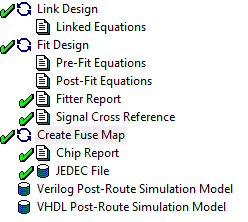
\includegraphics[scale = 0.85]{Graphics/Practice 1/ISPLever.PNG}
    \caption{ISPLever.}
    \label{fig:ISPLever}
\end{figure}

Due to the simplicity of the GAL, the pin assignments are automatically performed by the software, so we have to check which pins the compiler decided to use. To do this, we will make use of the \textbf{Chip Report} pop-up menu.

\begin{figure}[H]
    \centering
    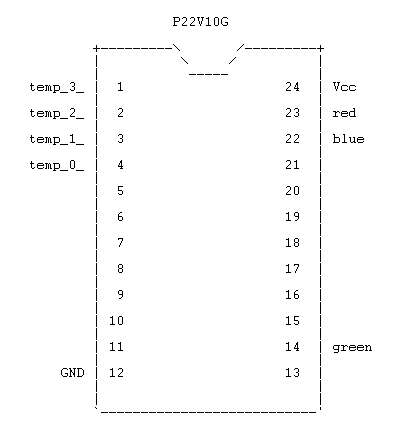
\includegraphics[scale=0.7]{Graphics/Practice 1/Chip_Report.PNG}
    \caption{Chip Report Output.}
    \label{fig:CHIP_REPORT}
\end{figure}

\newpage

Once everything checks, we will move on to simulating the circuit before finally assembling it. To do this, we will make use of ISIS Proteus, a well-know electronics simulation software.\medskip

Knowing the pin assignments makes the task of simulating the circuit very simple, as the only thing required is to follow the \textbf{Chip Report's} connections in Proteus.

\begin{figure}[H]
    \centering
    
    \ifnum\value{ANIMATION}=1 {
        \animategraphics[controls,loop,scale=1.2]{2}{Graphics/Practice 1/ANIMATION/F}{0}{15}
    } 
    \else {
        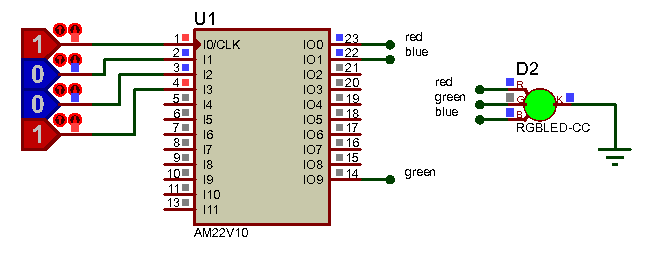
\includegraphics[scale=1.2]{Graphics/Practice 1/ANIMATION/F9.PDF}
    }\fi
    
    \caption{Proteus assembly.}
    \label{fig:PROTEUS_TEMP}
\end{figure}

Now that we have checked that the circuit works as intended, we can proceed to the real assembly. Again, this is just a matter of following the previous connections but this time using a protoboard and some hook-up wires. \medskip

As expected, everything worked great.

\newpage

\section{Laboratory Lecture 2: Flip Flops}

The main objective of this lab lecture is to learn about the operation of Flip Flops. In particular, we will discuss how JK flip flops work as well as some of their applications.

\subsection{Introduction}

A flip flop, also known as latch or bistable multivibrator, is a type of circuit that has two states, one of them represents a \textit{one} and the other one a \textit{zero}, i.e. a single bit of data. They are commonly used to store information in digital circuits.\medskip 

Flip flops can be edge-triggered, that is synchronous/clocked, or level triggered, that is asynchronous. In order to control them, we have to apply specific signals to the inputs, following their truth table.\medskip

Some examples of flip flops may include D Flip flops, D Latch Flip flops, SR Flip flops, and JK Flip flops, to name a few. In this practice we are going to work with the latter.

\subsubsection{JK Flip Flops}

Before diving into what a JK Flip Flop is, we will briefly talk about SR Flip Flops, as they are the old and troublesome early version of a JK one.\medskip

SR Flip Flops, also known as SR Latch, are one the most basic sequential logic circuits. They act as a one-bit memory, so a bistable device, that possesses 2 inputs. On the one hand, \textit{SET}, which will output a 1 and is usually labelled \textit{S}, and \textit{RESET}, which will output a 0, and is usually labelled \textit{R}. \medskip

Note than we can also find a clocked, or synchronous variation of the SR Flip Flop. The latter will have an extra input, \textit{CLK} and it will only trigger on the positive edge transitions of the clock.\medskip

Obviously, \textit{SR} stands for "Set-Reset". As we have previously said, the reset input resets the flip flop, that is, it makes the output, Q, go back to its original state of 0. The different input configurations will define the behaviour of the output following this fashion:\medskip


\begin{minipage}{\textwidth}
    \begin{minipage}[b]{0.49\textwidth}
        \centering
        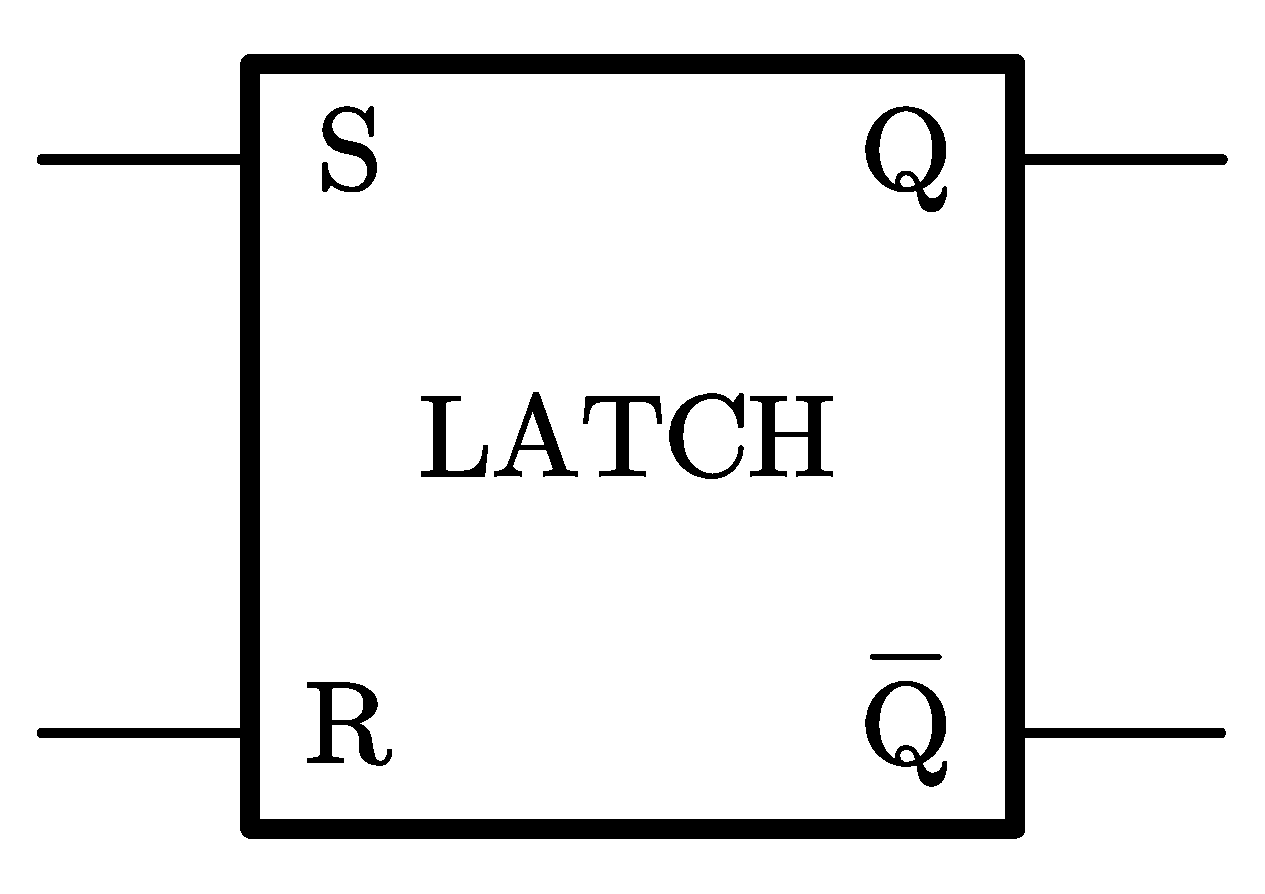
\includegraphics[scale=0.2]{Graphics/Practice 2/GRAPHICS/LOGIC GATES/SR ASYNCH.pdf}
        \captionof{figure}{SR Asynchronous Flip Flop.}
        \label{fig:SR_Asynch}
    \end{minipage}
    \hfill
    \begin{minipage}[b]{0.49\textwidth}
        \centering
             \begin{tabular}[t]{lccc}
                \toprule
                &\textbf{SET}&\textbf{RST}&\textbf{Q}\\
                \midrule
                & 0 & 0 & $Q_0 \text{ No change}$\\
                & 1 & 0 & Q = 1\\
                & 0 & 1 & Q = 0\\
                & 1 & 1 & Invalid\\
                \bottomrule
            \end{tabular}
        \captionof{table}{SR Flip Flop's Truth Table.}
    \end{minipage}
\end{minipage}\textbf{}

\clearpage

As we can deduce from the table, this type of flip flops pose a problem when both the \textit{S} and the \textit{R} inputs are 1, since the output state is invalid and cannot be predicted.\medskip

To solve this problem, we will make use of a \textbf{JK Flip Flop}. JK Flip flops, in a nutshell, solve this problem by having the output toggle when both inputs \textit{J} and \textit{K}, which correspond to the \textit{S} and \textit{R} terminals respectively, are 1. The truth table of this type of flip flop is as follows:\bigskip

\begin{minipage}{\textwidth}
    \begin{minipage}[b]{0.49\textwidth}
        \centering
        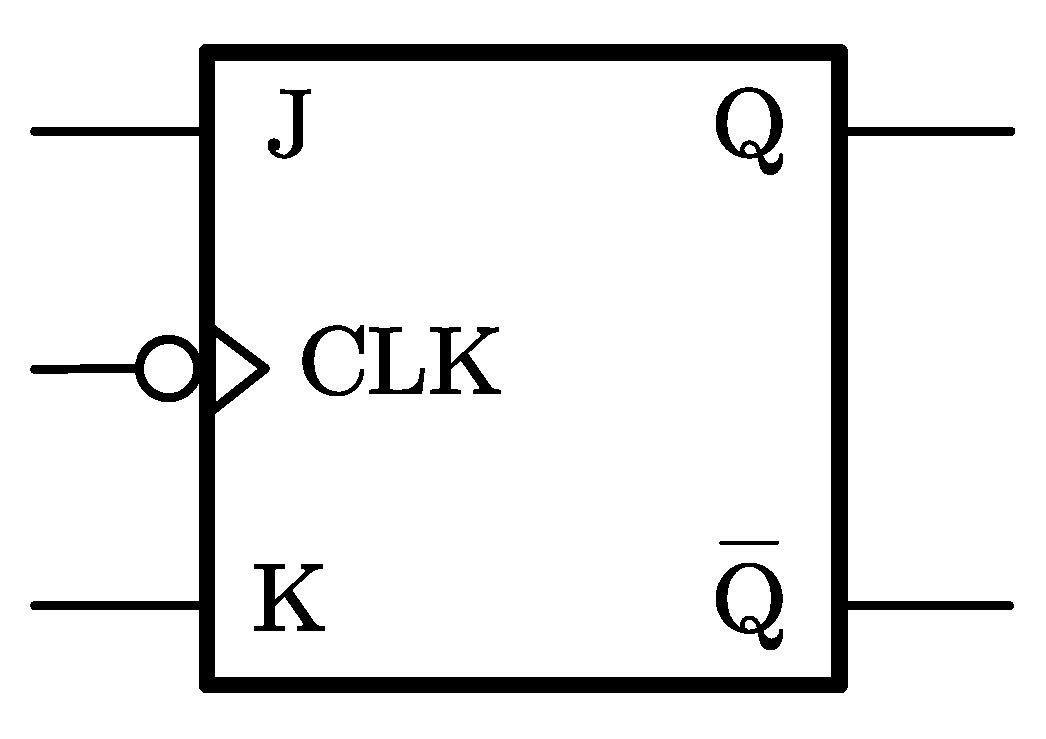
\includegraphics[scale=0.25]{Graphics/Practice 2/GRAPHICS/LOGIC GATES/JK SYNCH.pdf}
        \captionof{figure}{JK Synch. Flip Flop.}
        \label{fig:JK_Synch}
    \end{minipage}
    \hfill
    \begin{minipage}[b]{0.49\textwidth}
        \centering
            \begin{tabular}[t]{lcccc}
                \toprule
                &\textbf{J}&\textbf{K}&\textbf{CLK}&\textbf{Q}\\
                \midrule
                &0&0& $\uparrow$ & $Q_0 \text{ No change}$\\
                &1&0& $\uparrow$ & Q = 1\\
                &0&1& $\uparrow$ & Q = 0\\
                &1&1& $\uparrow$ & $\overline{Q_0} \text{ Toggles}$\\
                \bottomrule
            \end{tabular}
        \captionof{table}{JK's Synch. Truth Table.}
        \label{table:JK_Synch_TT}
    \end{minipage}
\end{minipage}

\vspace{0.5cm}

It is possible to find an asynchronous version of the JK Flip Flop as well. This version has two extra pins, \textit{PRESET} and \textit{CLEAR}, which, if active, will turn the output $Q$ to 0, if the \textit{PRESET} is connected to 1 and the \textit{CLEAR} to 0. Alternatively, they will turn the output $Q$ to 1 if the \textit{PRESET} is connected to 0, and the \textit{CLEAR} to 1. We can visualise this in the following truth table: 

\vspace{0.7cm}

\begin{minipage}{\textwidth}
    \begin{minipage}[b]{0.49\textwidth}
        \centering
        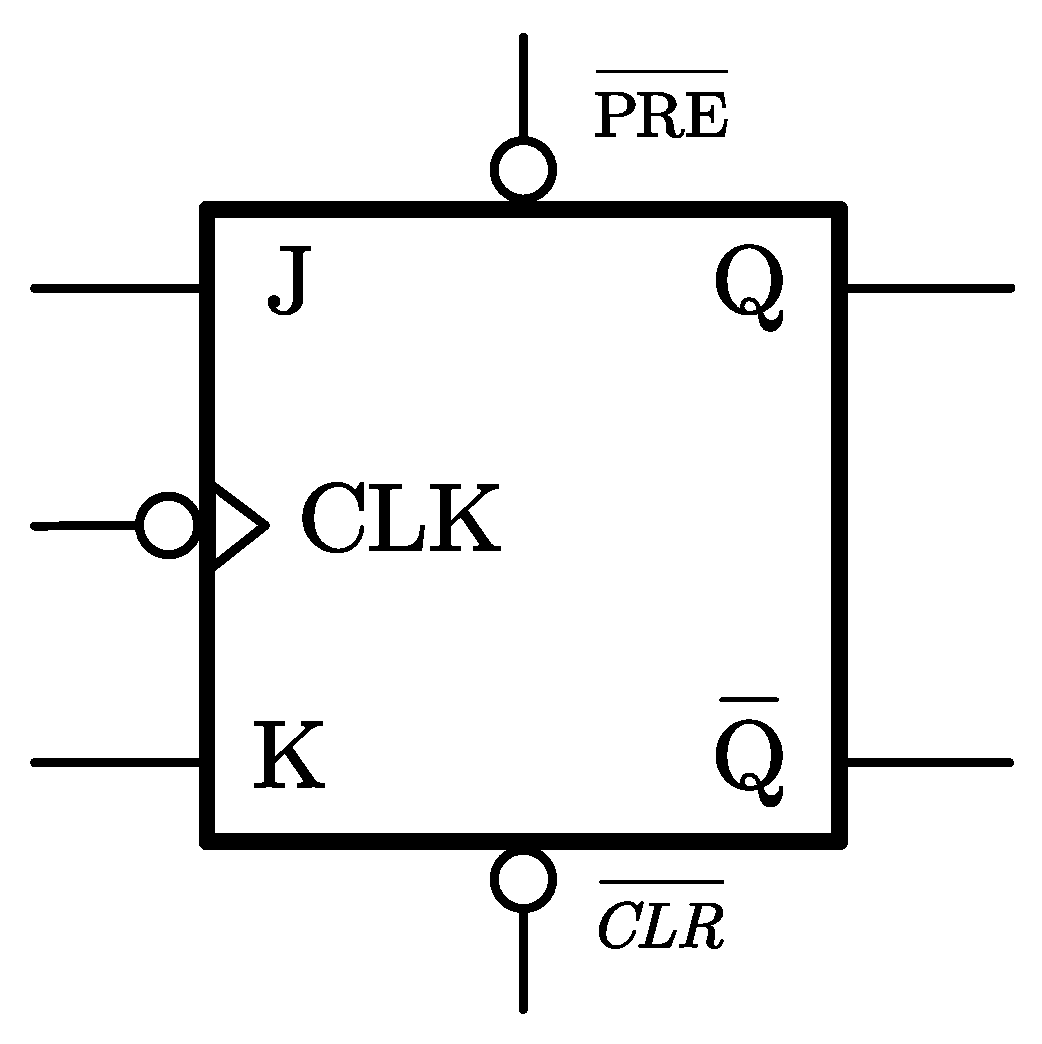
\includegraphics[scale=0.25]{Graphics/Practice 2/GRAPHICS/LOGIC GATES/JK ASYNCH.pdf}
        \captionof{figure}{JK Asynch. Flip Flop.}
        \label{fig:JK_Asynch}
    \end{minipage}
    \hfill
    \begin{minipage}[b]{0.49\textwidth}
        \centering
            \begin{tabular}[t]{lcccccc}
                \toprule
                & \textbf{J} & \textbf{K} & \textbf{CLK} & $\overline{\mathbf{PRE}}$ & $\overline{\mathbf{CLR}}$ & \textbf{Q}\\
                \midrule
                & 0 & 0 & $\downarrow$ & 1 & 1 & $Q_0$\\
                & 1 & 0 & $\downarrow$ & 1 & 1 & 1\\
                & 0 & 1 & $\downarrow$ & 1 & 1 & 0\\
                & 1 & 1 & $\downarrow$ & 1 & 1 & $\overline{Q_0}$\\
                \midrule
                & X & X & X & 0 & 0 & Inv\\
                & X & X & X & 0 & 1 & 1\\
                & X & X & X & 1 & 0 & 0\\
                \bottomrule
            \end{tabular}
        \captionof{table}{JK's Asynch. Truth Table.}
        \label{table:JK_Asynch_TT}
    \end{minipage}
\end{minipage}\textbf{}

\newpage

Now that we have established the basics, we will move on to completing the laboratory session.

\subsection{JK Synchronous Flip Flop}

\subsubsection{Asynchronous \textit{PRE} and \textit{CLR} effect on Q}

In order to complete this part, we will make use of the program Proteus, as per usual. We will simply follow Table \ref{table:JK_Asynch_TT} in order to check the output when \textit{PRE} and \textit{CLR} change.

\begin{figure}[H]
    \centering
    
    \ifnum\value{ANIMATION}=1 {
        \animategraphics[controls,loop,scale=1.4]{1}{Graphics/Practice 2/GRAPHICS/ANIMATION/JK ASYNCH/F}{0}{2}
    } 
    \else {
        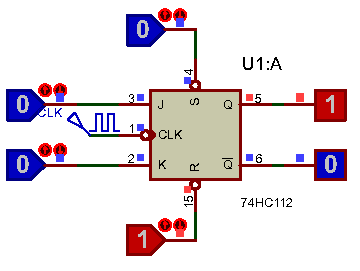
\includegraphics[scale=1.4]{Graphics/Practice 2/GRAPHICS/ANIMATION/JK ASYNCH/F1.PDF}
    }\fi
    
    \caption{Proteus assembly.}
    \label{fig:PROTEUS_JK_ASYNCH}
\end{figure}

In the simulation, we can not only see that the output, $Q$, is correct, but that it also does not depend on the values of \textit{J}, \textit{K}, and \textit{CLK}. 

\subsubsection{Synchronous \textit{J} and \textit{K} effect on Q}

For this part, as we are working with a Synchronous circuit, both \textit{PRE} and \textit{CLR} have to be tied to their inactive state, in this case, since they are active low, we will tie them to 1.

Again, we have to check that the circuit behaves as expected, that it, that it follows Table \ref{table:JK_Synch_TT}

\newpage

To achieve this, we will use Proteus once more.

\begin{figure}[H]
    \centering
    
    \ifnum\value{ANIMATION}=1 {
        \animategraphics[controls,loop,scale=1.4]{1}{Graphics/Practice 2/GRAPHICS/ANIMATION/JK SYNCH/F}{0}{5}
    } 
    \else {
        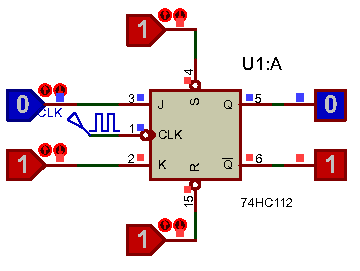
\includegraphics[scale=1.4]{Graphics/Practice 2/GRAPHICS/ANIMATION/JK SYNCH/F2.PDF}
    }\fi
    
    \caption{Proteus assembly.}
    \label{fig:PROTEUS_JK_SYNCH}
\end{figure}

As we can see, the circuit behaves as expected.


\subsection{T Flip Flop from JK Flip Flop}

In this exercise we are asked to create a T Flip Flop using a JK one. To do this we have to take Table \ref{table:JK_Synch_TT} into account, as it clearly states that when both inputs, \textit{J} and \textit{K} are tied to 1, and a falling edge of the clock occurs -in the case of a 74HC112-, the output toggles, which is precisely what we aim to obtain.


\begin{figure}[H]
    \centering
    
    \ifnum\value{ANIMATION}=1 {
        \animategraphics[controls,loop,scale=1.4]{2}{Graphics/Practice 2/GRAPHICS/ANIMATION/T/F}{0}{1}
    } 
    \else {
        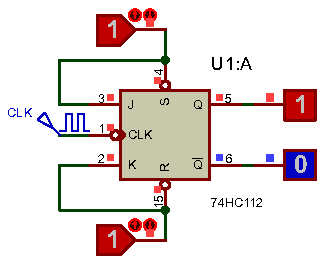
\includegraphics[scale=1.4]{Graphics/Practice 2/GRAPHICS/ANIMATION/T/F1.PDF}
    }\fi
    
    \caption{Proteus assembly.}
    \label{fig:PROTEUS_T}
\end{figure}

\clearpage

One of the most important applications of this type of gate is to build a frequency divider. Since we are using a 74HC112 as a T Flip Flop, if we apply a \textit{CLK} signal with a duty cycle of $50\%$ to the clock input, the output $Q$ will toggle every time a falling edge occurs, that is, every full cycle, effectively dividing the input frequency by 2. We can visualise this in the following timing diagram: \medskip

\begin{figure}[H]
    \centering
    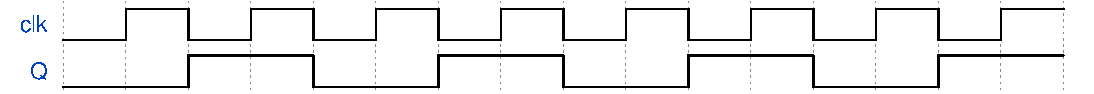
\includegraphics[scale = 0.73]{Graphics/Practice 2/GRAPHICS/TIMING/EX2.pdf}
    \caption{Timing diagram of a 2-bit frequency divider.}
    \label{fig:timing_1}
\end{figure}

\subsection{T Flip Flop Asynchronous counter}

Now that we have established how to build a frequency divider, we will focus on its applications. In particular, we will build a binary counter, which will be fed to a BCD to 7 segment display decoder, so as to help us visualise the output.\medskip

In Figure \ref{fig:timing_1}, we can already see the the behaviour that we are aiming for. In the first division, the \textit{Q} and the \textit{clk} signals have a logic level of 0, or 00 in binary. This value turns into a 01 in the second division, 10, in the third, and finally 11 in the fourth. Translating these numbers into decimal yields 0, 1, 2, 3, so we can say that Figure \ref{fig:timing_1} represents a 2 bit binary counter.\medskip

In order to be able to display numbers up to 7, we will need a 3 bit binary counter. Building it is just a matter of concatenating 2 T Flips Flops following this fashion:

\begin{figure}[H]
    \centering
    
    \ifnum\value{ANIMATION}=1 {
        \animategraphics[controls,loop,scale=0.85]{2}{Graphics/Practice 2/GRAPHICS/ANIMATION/7_SEG/F}{0}{7}
    } 
    \else {
        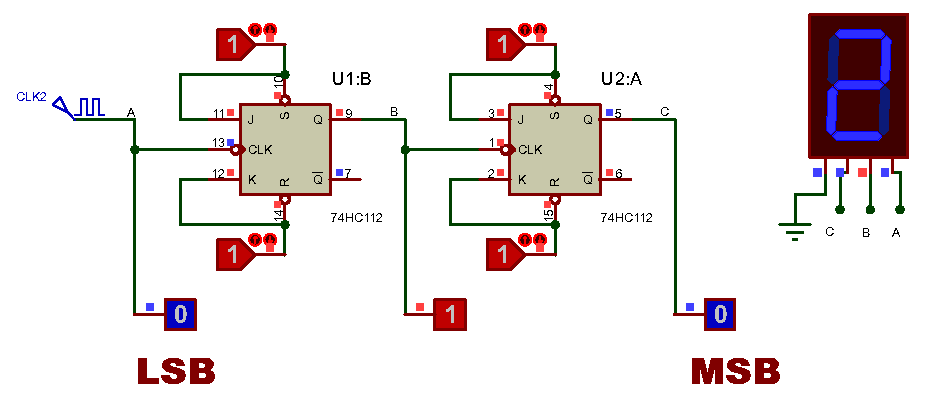
\includegraphics[scale=0.85]{Graphics/Practice 2/GRAPHICS/ANIMATION/7_SEG/F2.PDF}
    }\fi
    
    \caption{Proteus assembly.}
    \label{fig:PROTEUS_7_SEG}
\end{figure}

\clearpage

If we look at the output signals with a logic analyser, we will see the following:\medskip

\begin{figure}[H]
    \centering
    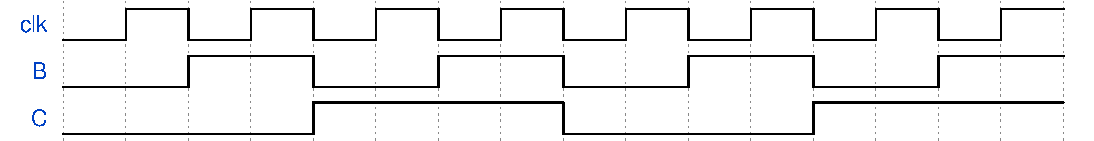
\includegraphics[scale = 0.73]{Graphics/Practice 2/GRAPHICS/TIMING/EX3.pdf}
    \caption{Timing diagram of a 3-bit frequency divider.}
    \label{fig:timing_2}
\end{figure}

The only problem that this configuration poses, is that a small glitch is produced at the output due to the propagation time of the \textit{CLK} signals, as the output of the first T Flip Flop is fed into the input of the next one and so on.\medskip 

One possible solution would be to add a capacitor connected to ground to each of the 3 outputs, in order to smooth out the peak and make the transition more visually appealing and less prone to error.

\clearpage

\section{Laboratory Lecture 2 BIS: 555 Timer}

\subsection{Introduction}

Up until this point we have seen how to manipulate clock signals by using frequency dividers, but what if we want to obtain a specific type of output response, for instance a single pulse or a clock with a duty cycle different from 50\% ? In this case, a multivibrator circuit is needed. \medskip

These type of integrated circuits use an RC timer to set the pulse duration and, depending on the manufacturer, they may work in different modes, i.e.:

\begin{enumerate}
    \item Clock generator circuits (Astable Multivibrator)
    
    \item One-Shot (Monostable Multivibrator)
    \begin{itemize}
        \item Retriggerable
        \item Non-Retriggerable
    \end{itemize}
\end{enumerate}

\subsubsection{Astable Multivibrator}

The first type of circuit, the \textbf{Astable Multivibrator}, is what is commonly referred to as \textbf{"Clock"}. These simple circuits basically switch back and forth between two unstable states with a specific duty cycle\footnote{The duty cycle of a digital circuit is the percentage of the ratio of pulse duration, or pulse width to the total period. It can be expressed as: 

\begin{equation*}
    D = \frac{t_{ON}}{t_{ON} + t_{OFF}} \cdot 100
    \label{fig:DUTY}
\end{equation*}
} set by an RC circuit. \medskip

In the previous section we have seen how modify a clock signal to obtain a specific output frequency, taking into account the limitations of an even division of course. The problem with this type of circuits is that they cannot provide custom duty cycles, which are needed in real case scenarios. That is when astable circuits come in handy.\medskip

\subsubsection{Monostable Multivibrator}

On the other hand, we can also find \textbf{Monostable Multivibrators}, commonly referred to as \textbf{"One-Shots"}. These type of circuits, as the name suggests, only output a single pulse when triggered, that is, they have only one stable state. The change from stable to quasi-stable occurs for a fixed time period $\mathbf{t_{p}}$ or $\mathbf{t_{w}}$ which is determined by an RC constant as well.\medskip

These circuits are readily available and they usually come in two forms, i.e. a retriggerable and a non-retriggerable one. When a retriggerable one-shot is triggered before the end of the pulse, the pulse duration $\mathbf{t_{p}}$, is restarted. Contrarily, when a non-retriggerable monostable is triggered before the end of the pulse, the output remains the same, in other words, the input is ignored until the output returns to the steady state.\medskip


\clearpage

We can visualise their behaviour in the following graphs:

\begin{figure}[H]
    \centering
    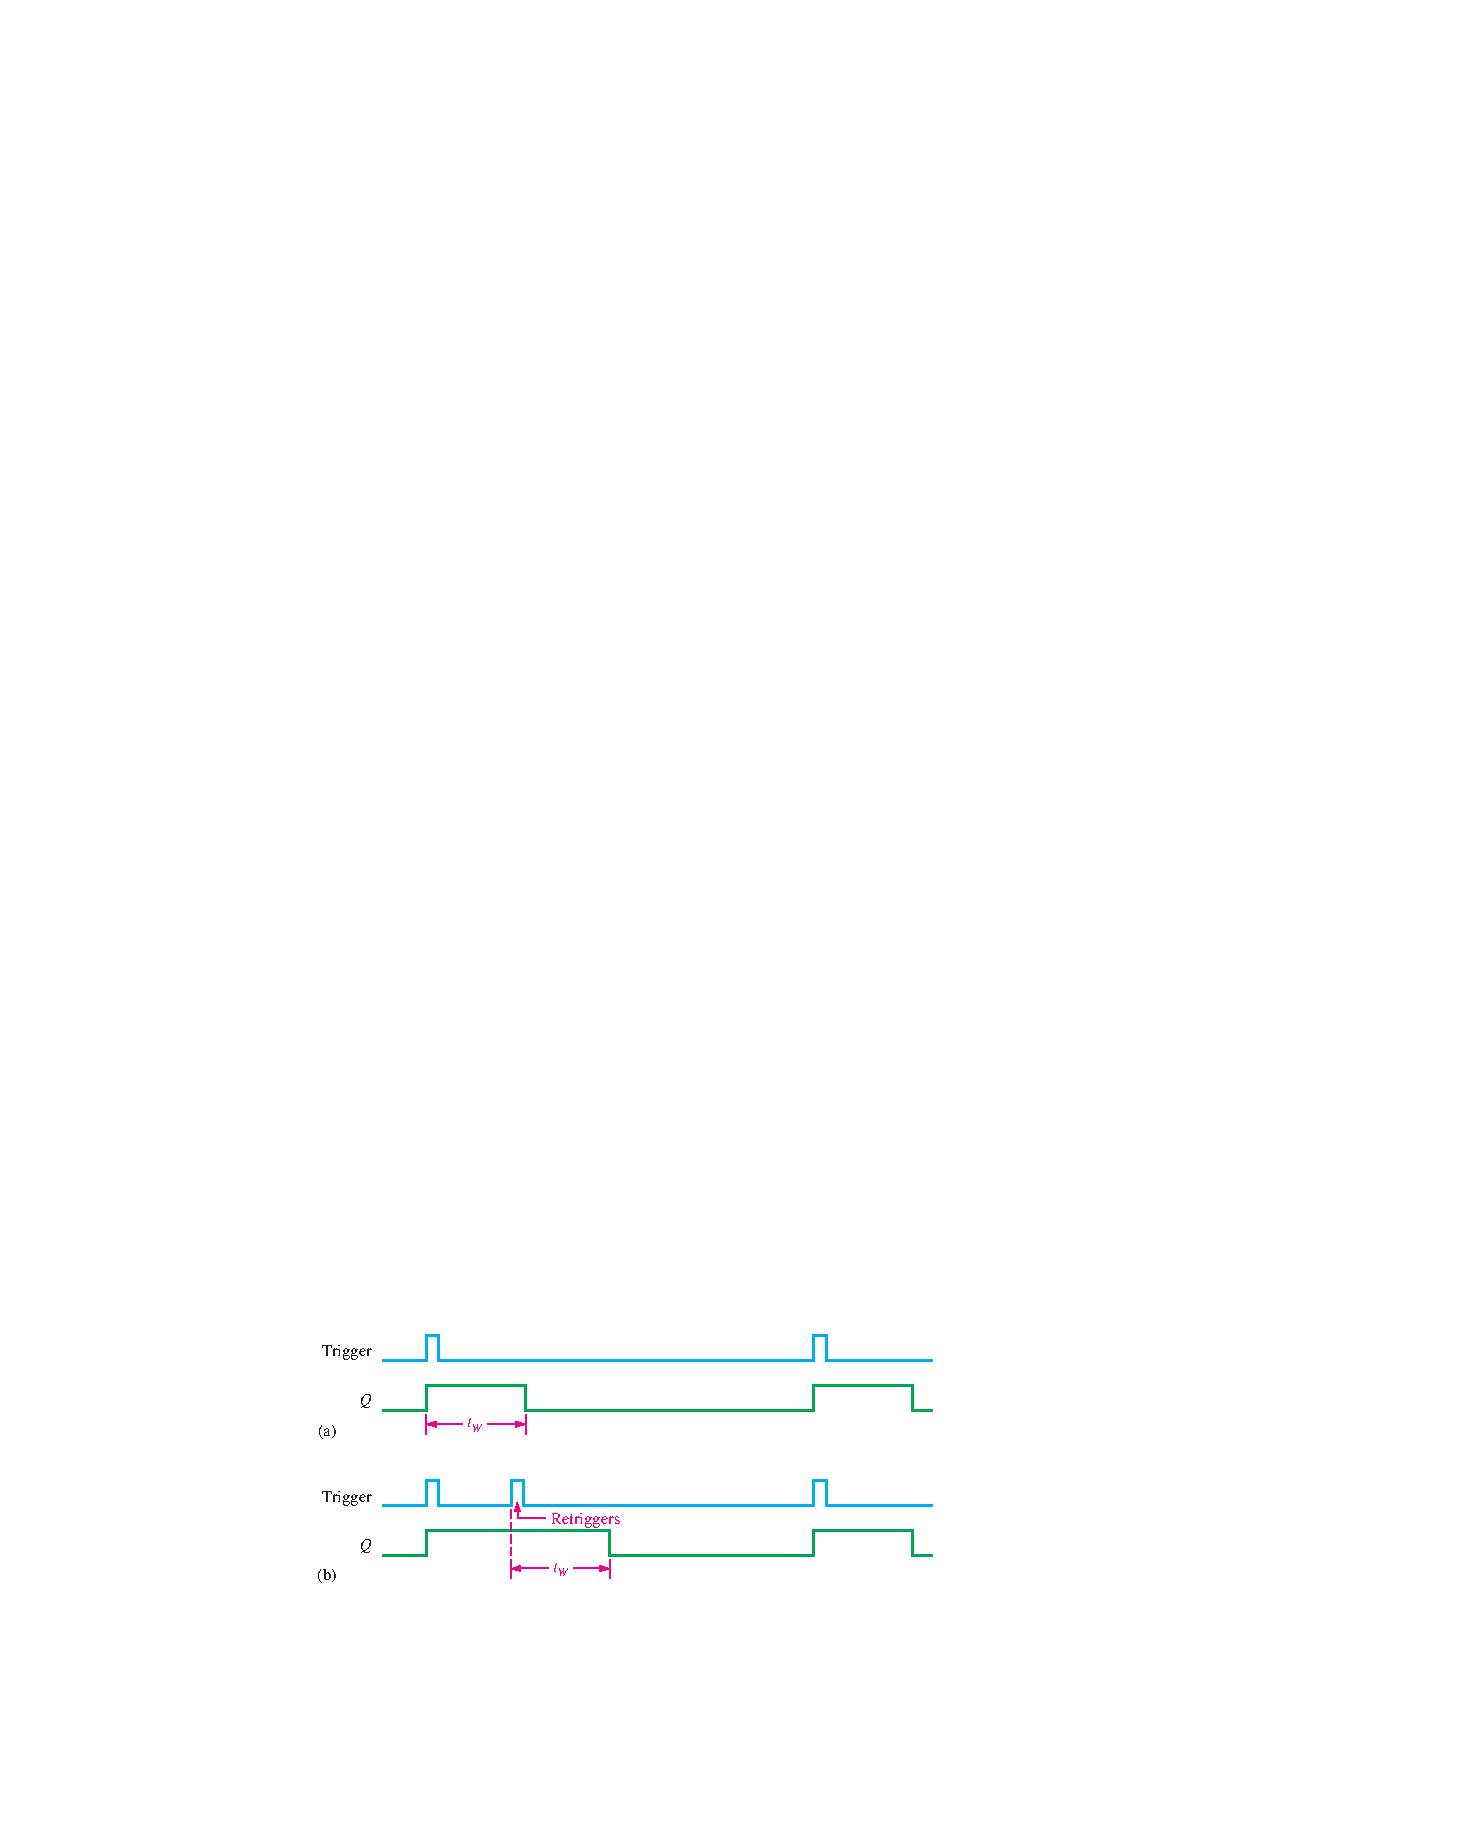
\includegraphics[scale = 1]{Graphics/Practice 2/GRAPHICS/MONOSTABLE/RETRIGGERABLE.pdf}
    \caption{Retriggerable Monostable. ~\autocite{FLOYD}}
    \label{fig:RETRIGGERABLE}
\end{figure}

\begin{figure}[H]
    \centering
    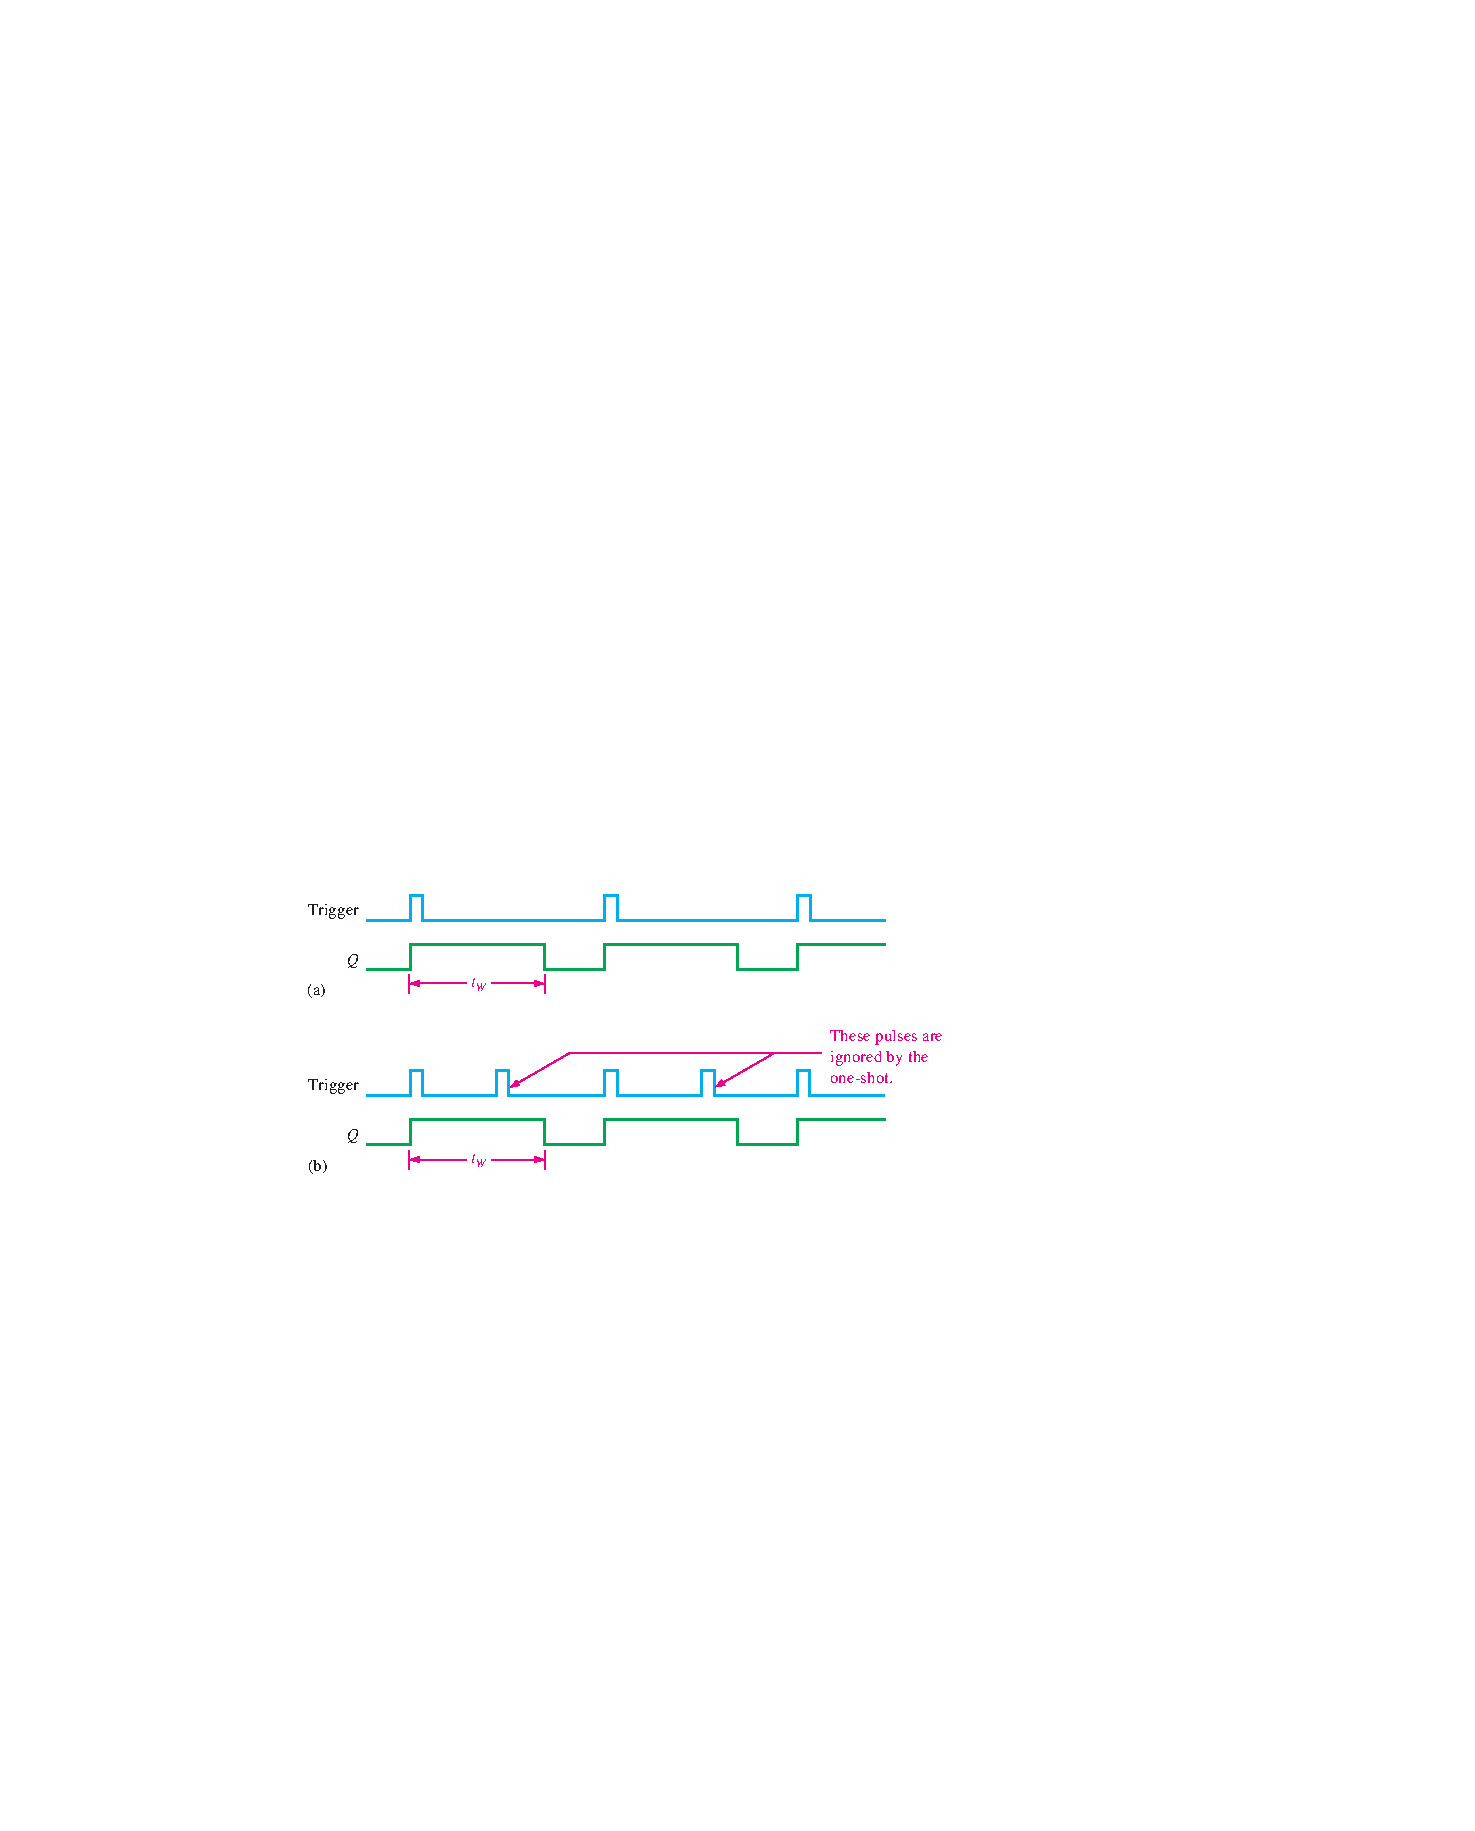
\includegraphics[scale = 1]{Graphics/Practice 2/GRAPHICS/MONOSTABLE/NON-RETRIGGERABLE.pdf}
    \caption{Non-Retriggerable Monostable. ~\autocite{FLOYD}}
    \label{fig:NON-RETRIGGERABLE}
\end{figure}


Both monostables, as well as the astable one, can be implemented using VHDL, but we will not dive into this, as it is not required in this practice, though they can be found \href{https://drive.google.com/open?id=1J-T80ZyF3isizOMjBf8xZOD7rw0KesP-}{\textbf{here}}.

\clearpage

\subsection{555 Timer}

Now that every type of multivibrator has been introduced, we will discuss the 555 timer. This timer is a TTL-compatible device that can operate in both of the modes described above. The heart of the 555 timer is composed of two voltage comparators and a SR Latch (See \ref{fig:SR_Asynch}). \medskip

The comparators are devices whose outputs are HIGH when the voltage on the positive (\texttt{+}) input is greater than the voltage on the negative (\texttt{-}) input and LOW when the (\texttt{-}) input voltage is greater than the (\texttt{+}) input voltage. \medskip

The voltage divider consisting of three 5 k$\Omega$ resistors provides a trigger level of $\frac{1}{3}$ VCC and a threshold level of $\frac{2}{3}$ VCC. The control voltage input (pin 5) can be used to externally adjust the trigger and threshold levels to other values if necessary.\medskip 

When the normally HIGH trigger input momentarily goes below $\frac{1}{3}$ VCC, the output of comparator B switches from LOW to HIGH and sets the S-R latch, causing the output (pin 3) to go HIGH and turning the discharge transistor Q1 off.\medskip

The output will stay HIGH until the normally LOW threshold input goes above $\frac{2}{3}$ VCC and
causes the output of comparator A to switch from LOW to HIGH. This resets the latch,
causing the output to go back LOW and turning the discharge transistor on. The external
reset input can be used to reset the latch independent of the threshold circuit. The trigger
and threshold inputs (pins 2 and 6) are controlled by external components connected to
produce either monostable or astable action. ~\autocite{FLOYD}


\begin{figure}[H]
    \centering
    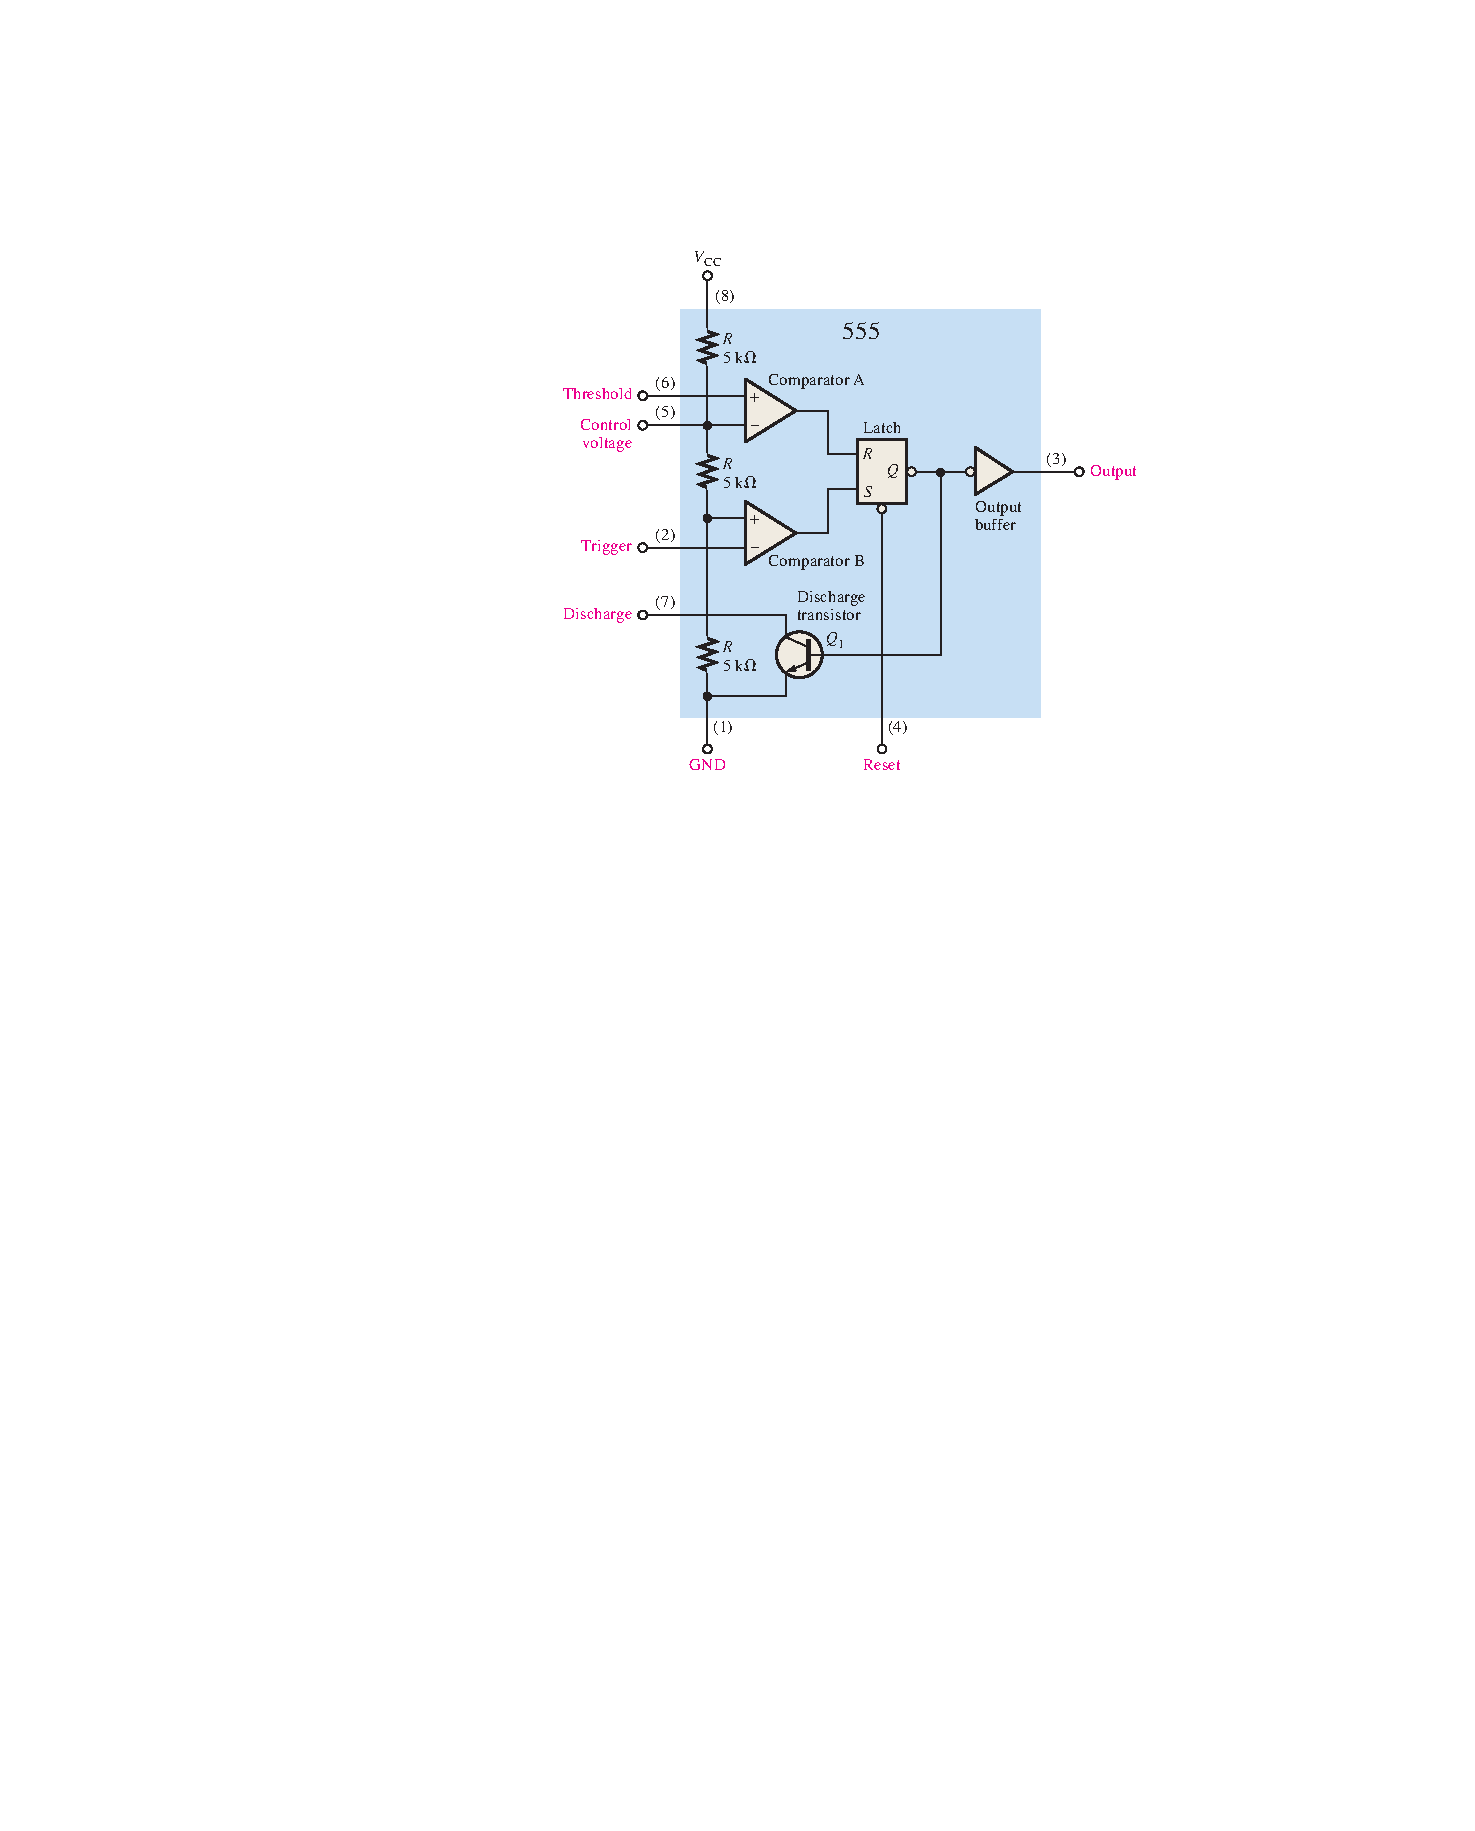
\includegraphics[scale = 0.99]{Graphics/Practice 2/GRAPHICS/555/GRAPHS/DATASHEETS/555_INTERNALS.pdf}
    \caption{Internal functional diagram of a 555 timer. ~\autocite{FLOYD}}
    \label{fig:555_DIAGRAM}
\end{figure}


\subsubsection{Astable 555}

As we have mentioned before, the 555 timer can be configured as a basic \textbf{Astable Multivibrator} following the circuit down below:

\begin{figure}[H]
    \centering
    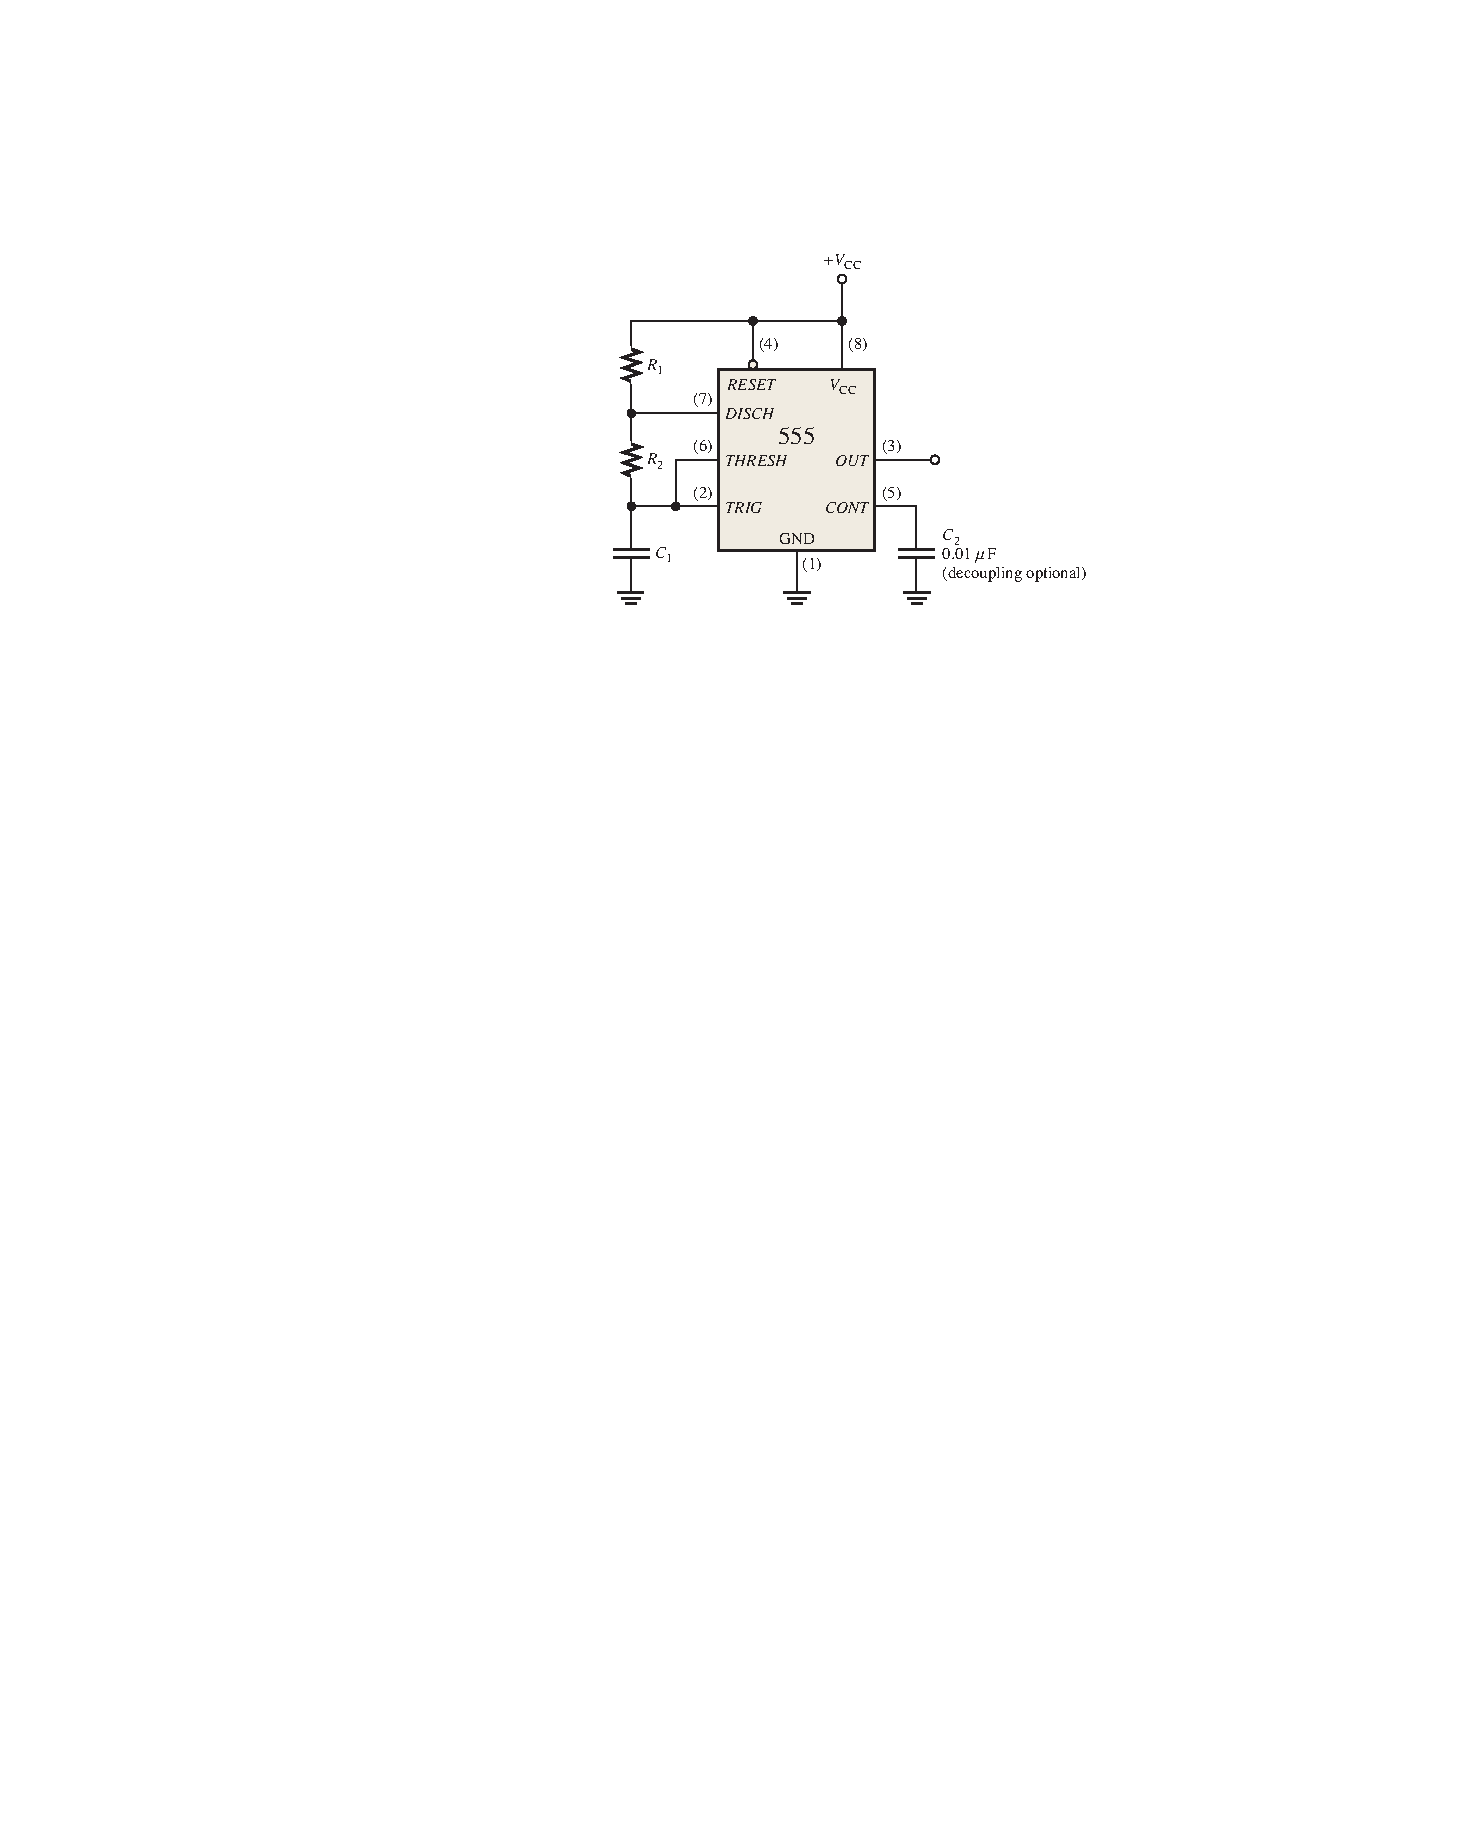
\includegraphics[scale = 1]{Graphics/Practice 2/GRAPHICS/555/GRAPHS/MODES/ASTABLE.pdf}
    \caption{555 timer connected as an astable multivibrator (oscillator). ~\autocite{FLOYD}}
    \label{fig:ASTABLE}
\end{figure}

In this circuit C1 charges through R1 and R2 and discharges through only R2. The output frequency is given by:

\begin{equation*}
    f = \frac{1.44}{(R_1 + 2\cdot R_2) \cdot C_1}
\end{equation*}

\vspace{0.25cm}

In order to help us find a set of suitable component values, the manufacturer provides a chart that shows sets of compatible and valid configurations. Besides, some useful equations are provided:

\vspace{0.6cm}

\begin{minipage}{\textwidth}
    \begin{minipage}[c]{0.49\textwidth}
        \centering
        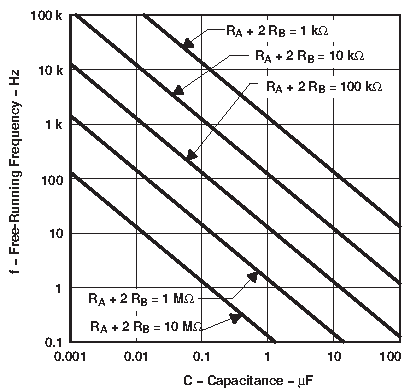
\includegraphics[scale=1]{Graphics/Practice 2/GRAPHICS/555/GRAPHS/DATASHEETS/ASTABLE_FREQ.pdf}
        \captionof{figure}{555 Astable Freq. Chart. ~\autocite{555_DS}}
        \label{fig:ASTABLE_FREQ}
    \end{minipage}
    \hfill
    \begin{minipage}[c]{0.49\textwidth}
        \centering
            \begin{align*}
                t_H &= 0.693 \cdot (R_1 + R_2) \cdot C_1& \\
                t_L &= 0.693 \cdot (R_2) \cdot C_1& \\
                T &= 0.693 \cdot (R_1 + 2\cdot R_2) \cdot C_1& \\
            \end{align*}
            
            \vspace{1.5cm}
    \end{minipage}
\end{minipage}

    
\subsubsection{Monostable 555}

The 555 timer can also be used as a \textbf{Monostable Multivibrator} following the circuit down below. 

\begin{figure}[H]
    \centering
    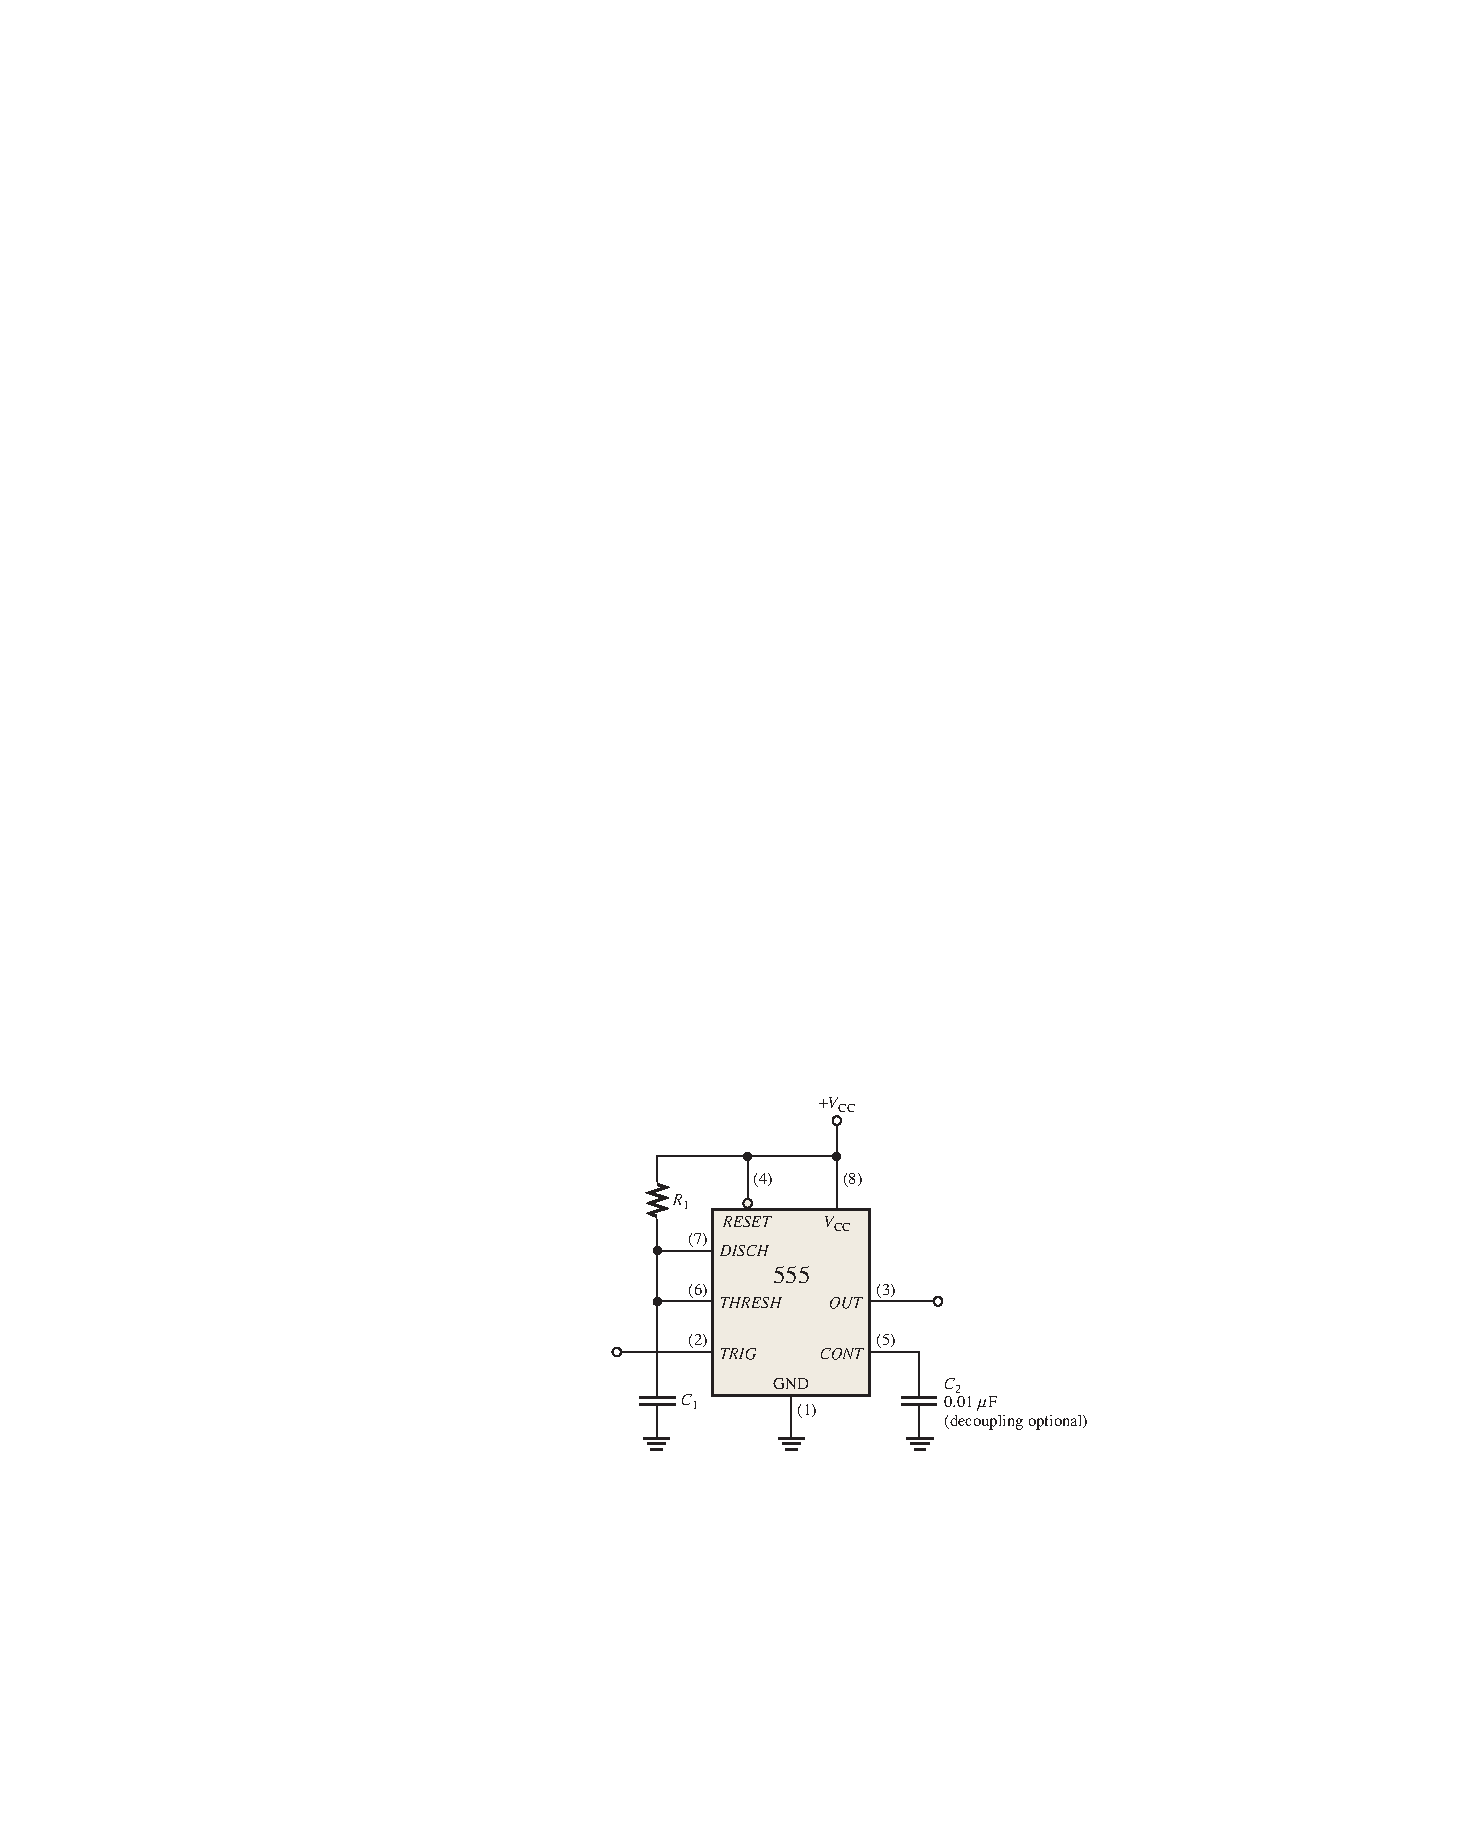
\includegraphics[scale = 1]{Graphics/Practice 2/GRAPHICS/555/GRAPHS/MODES/MONOSTABLE.pdf}
    \caption{555 timer connected as an monostable multivibrator (One-shot). ~\autocite{FLOYD}}
    \label{fig:MONOSTABLE}
\end{figure}

As per the other configuration, the duration of the pulse $\mathbf{t_{p}}$ or $\mathbf{t_{w}}$ can be determined by the next equation:

\begin{equation*}
    t_{p} = 1.1 \cdot R_1 \cdot C_1
\end{equation*}

For this configuration, the trigger is a NGP (Negative-going pulse). In the manufacturer's datasheet we can find a chart similar to the last one: \medskip

\begin{figure}[H]
    \centering
    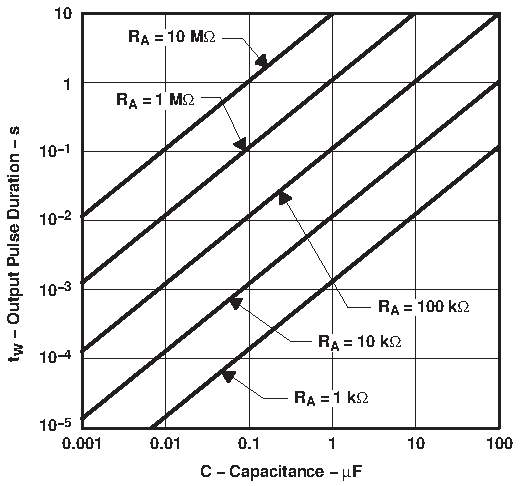
\includegraphics[scale = 0.8]{Graphics/Practice 2/GRAPHICS/555/GRAPHS/DATASHEETS/MONOSTABLE_FREQ.pdf}
    \caption{555 timer Monostable Frequency Chart. ~\autocite{555_DS}}
    \label{fig:MONOSTABLE_FREQ}
\end{figure}

\clearpage


\subsection{Exercise 1: 555 as Astable Multivibrator}

\textit{Design an astable multivibrator by using 555 timer with C = 10 nF, $R_1$ = 10 k$\Omega$ y $R_2$ = 10 k$\Omega$. Calculate theoretically the value of $t_H$ (high level semi period), T (period) and DC\% (duty cycle).}\medskip

\textit{Draw and simulate the circuit. Obtain the graphics of the outputs and between the pins of the capacitor. Measure the values of $t_H$ (high level semi period), T (period) and DC\% (duty cycle).}\bigskip

\textbf{\large Answer to Exercise 1:}\medskip

Using the equations listed in \ref{fig:ASTABLE_FREQ} and \ref{fig:DUTY}, obtaining what we are asked is rather simple:

\vspace{-.5cm}

\begin{align*}
    \mathbf{t_H} &= 0.693 \cdot (R_1 + R_2) \cdot C_1 = 0.693 \cdot (10k\Omega + 10k\Omega) \cdot 10\si\nano \text{F} = \mathbf{138.6 \, \textbf{\si\micro s}}
    \\
    \mathbf{t_L} &= 0.693 \cdot (R_2) \cdot C_1 = 0.693 \cdot (10k\Omega) \cdot 10\si\nano \text{F} = \mathbf{69.3 \, \textbf{\si\micro s}}
    \\
    \mathbf{T} &= t_L + t_H = \mathbf{207.9 \, \si\micro \text{s}}
    \\
    \mathbf{D} &= \frac{t_H}{t_H + t_L} \cdot 100= \frac{\mathbf{138.6 \, \si\micro \text{s}}}{\mathbf{138.6 \, \si\micro \text{s} + \mathbf{69.3 \, \textbf{\si\micro s}}}} \cdot 100 = \mathbf{66.6 \, \text{\%}}
\end{align*}\medskip

We are also asked to simulate the circuit. To do this we will make use of ISIS Proteus, as we have done in the past. 

\begin{figure}[H]
    \centering
    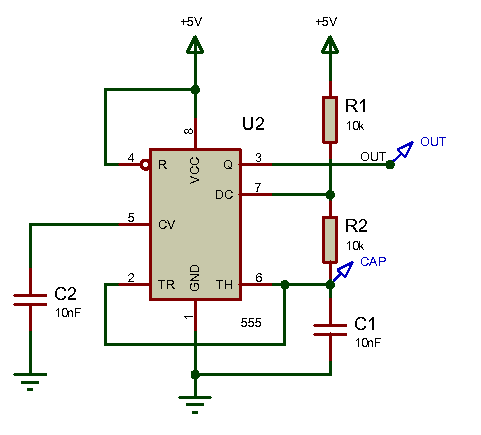
\includegraphics[scale = 1.1]{Graphics/Practice 2/GRAPHICS/555/GRAPHS/PROTEUS/ASSEMBLY/555_ASTABLE_10K_ASSEMBLY.PDF}
    \caption{Proteus assembly of the first subsection with $R_2 = 10k \Omega$.}
    \label{fig:555_ASTABLE_10K_ASSEMBLY}
\end{figure}

\clearpage

To check the output, we will employ the Analogue Analysis tool:

\begin{figure}[H]
    \centering
    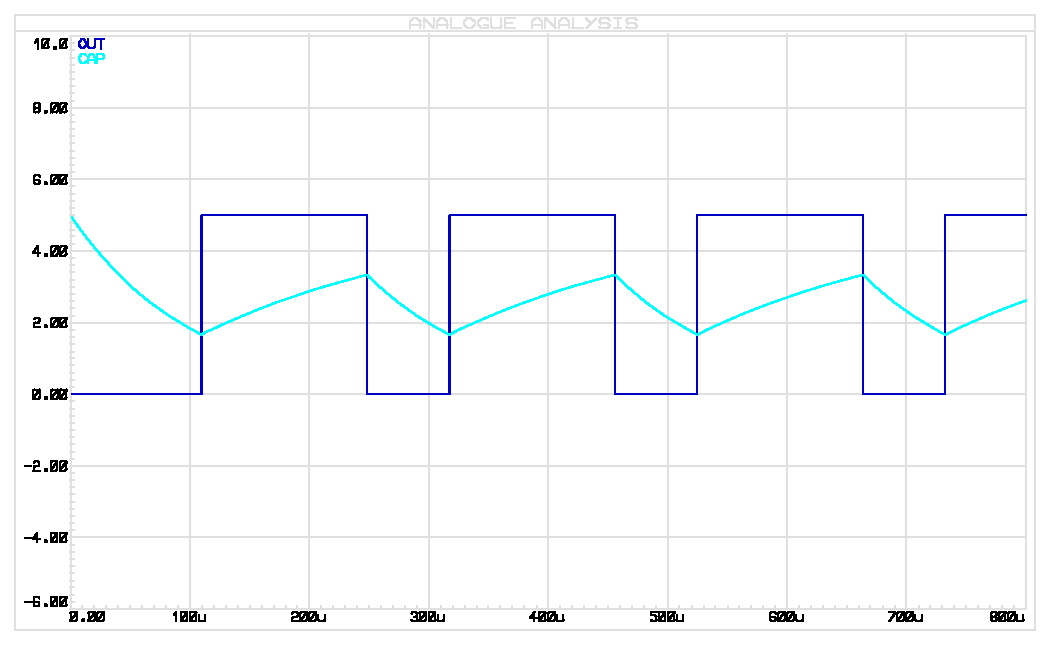
\includegraphics[scale = 0.75]{Graphics/Practice 2/GRAPHICS/555/GRAPHS/PROTEUS/ANALOGUE/555_ASTABLE_ANALOGUE_10K.PDF}
    \caption{Analogue Analysis of circuit with $R_2 = 10k \Omega$.}
    \label{fig:555_ASTABLE_ANALOGUE_10K}
\end{figure}


Using the cursors, we can measure the required parameters:

\begin{equation*}
    \mathbf{t_H} = \mathbf{207 \, \si\micro \text{s}} \quad
    \mathbf{t_L} = \mathbf{69 \, \si\micro \text{s}} \quad
    \mathbf{T} = \mathbf{207 \, \si\micro \text{s}} \quad
    \mathbf{D} =  \mathbf{66.6 \, \text{\%}}
\end{equation*}\medskip

As we can see, they match the calculations perfectly since proteus doesn't take into account the tolerances of the different components. The same simulation in NI Multisim yields vastly different results, due to its mathematical models of components being more accurate.\medskip

\clearpage

The exercise now asks us to change the value of $R_2$ to $100k\Omega$ and measure the same parameters. After following the same procedure, we obtain these results:

\begin{figure}[H]
    \centering
    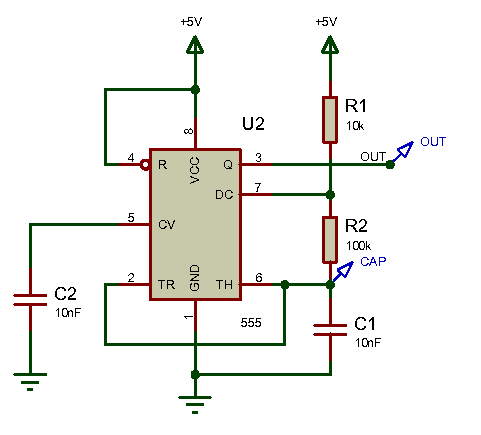
\includegraphics[scale = 1.1]{Graphics/Practice 2/GRAPHICS/555/GRAPHS/PROTEUS/ASSEMBLY/555_ASTABLE_100K_ASSEMBLY.PDF}
    \caption{Proteus assembly of the second subsection with $R_2 = 100k \Omega$.}
    \label{fig:555_ASTABLE_100K_ASSEMBLY}
\end{figure}

\begin{figure}[H]
    \centering
    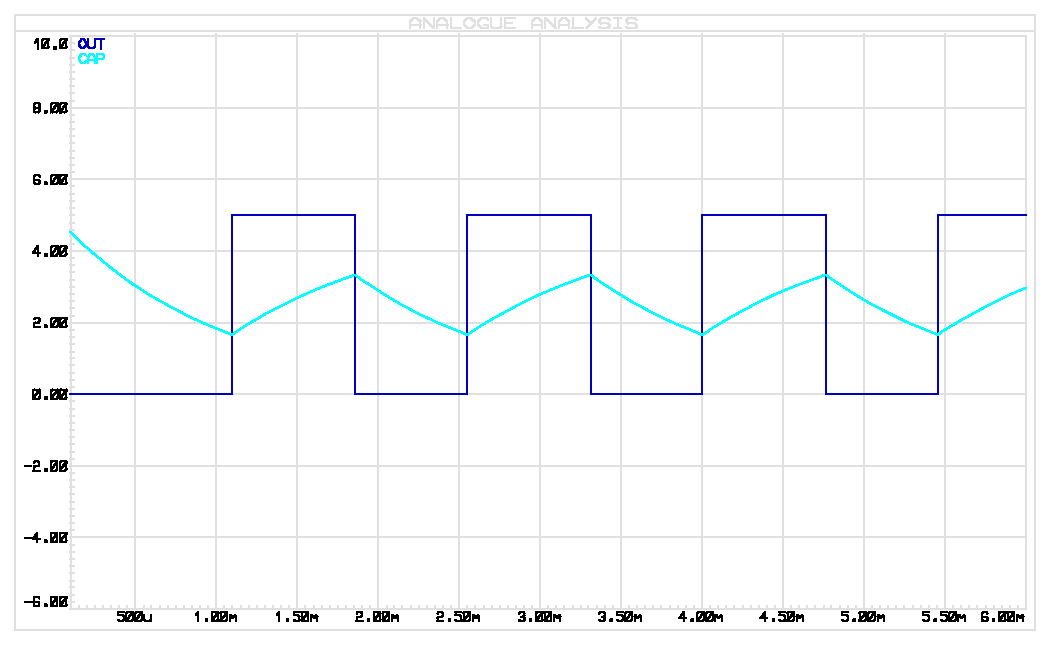
\includegraphics[scale = 0.75]{Graphics/Practice 2/GRAPHICS/555/GRAPHS/PROTEUS/ANALOGUE/555_ASTABLE_ANALOGUE_100K.PDF}
    \caption{Analogue Analysis of circuit with $R_2 = 100k \Omega$.}
    \label{fig:555_ASTABLE_ANALOGUE_100K}
\end{figure}

\vspace{-.4cm}

\begin{equation*}
    \mathbf{t_H} = \mathbf{762 \, \si\micro \text{s}} \quad
    \mathbf{t_L} = \mathbf{693 \, \si\micro \text{s}} \quad
    \mathbf{T} = \mathbf{1455 \, \si\micro \text{s}} \quad
    \mathbf{D} =  \mathbf{52.37 \, \text{\%}}
\end{equation*}
\clearpage


The exercise finally asks us to add a diode in parallel with $R_2$ and measure the same parameters. After following the same procedure, we obtain these results:

\begin{figure}[H]
    \centering
    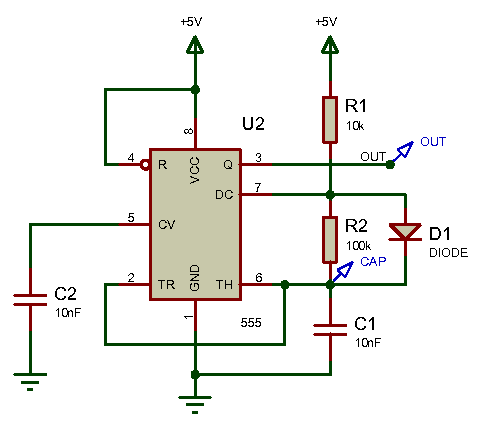
\includegraphics[scale = 1.1]{Graphics/Practice 2/GRAPHICS/555/GRAPHS/PROTEUS/ASSEMBLY/555_ASTABLE_100K_DIODE_ASSEMBLY.PDF}
    \caption{Proteus assembly of the third subsection with $R_2 = 100k \Omega$ and a diode in parallel.}
    \label{fig:555_100K_DIODE}
\end{figure}


\begin{figure}[H]
    \centering
    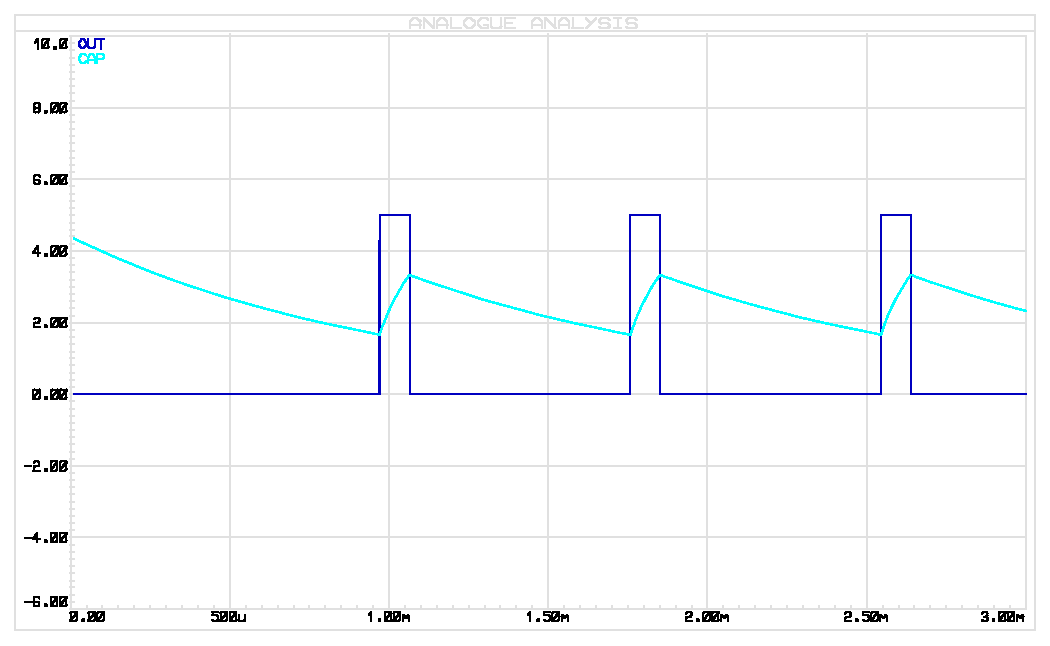
\includegraphics[scale = 0.8]{Graphics/Practice 2/GRAPHICS/555/GRAPHS/PROTEUS/ANALOGUE/555_ASTABLE_ANALOGUE_100K_DIODE.PDF}
    \caption{Analogue Analysis with $R_2 = 100k\Omega$ and Diode in parallel.}
    \label{fig:555_ANALOGUE_100K_DIODE}
\end{figure}

\vspace{-.4cm}

\begin{equation*}
    \mathbf{t_H} = \mathbf{98 \, \si\micro \text{s}} \quad
    \mathbf{t_L} = \mathbf{690 \, \si\micro \text{s}} \quad
    \mathbf{T} = \mathbf{788 \, \si\micro \text{s}} \quad
    \mathbf{D} =  \mathbf{12.44 \, \text{\%}} 
\end{equation*}


\subsection{Exercise 2: 555 as Monostable Multivibrator}

In this exercise we are asked to design a one-shot multivibrator (Figure \ref{fig:MONOSTABLE} )using a 555 timer, a 10 \si\micro F capacitor and a $100k\Omega$ resistor. As a reminder, the duration of the pulse of a 555 monostable can be obtained using this equation:

\begin{equation*}
    t_{p} = 1.1 \cdot R_1 \cdot C_1 = 1.1 \cdot 100k\Omega \cdot 10 \si\micro \text{F} = 1.10 \text{s}
\end{equation*}


\begin{figure}[H]
    \centering
    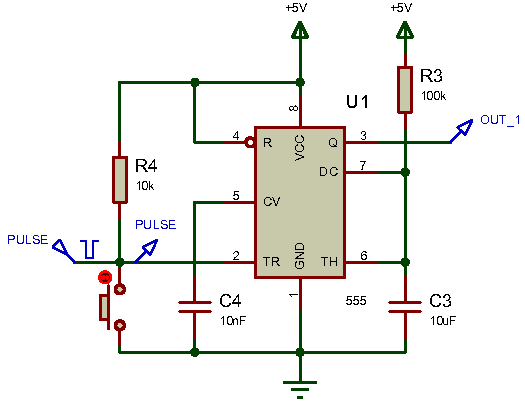
\includegraphics[scale = 1.045]{Graphics/Practice 2/GRAPHICS/555/GRAPHS/PROTEUS/ASSEMBLY/555_MONO_ASSEMBLY.PDF}
    \caption{Proteus assembly of a Monostable Multivibrator}
    \label{fig:555_MONO_ASSEMBLY}
\end{figure}


\begin{figure}[H]
    \centering
    
    \ifnum\value{ANIMATION}=1 {
        \animategraphics[controls,loop,scale=0.75]{1}{Graphics/Practice 2/GRAPHICS/ANIMATION/555/555_MONO_ANALOGUE_F}{0}{1}
    } 
    \else {
        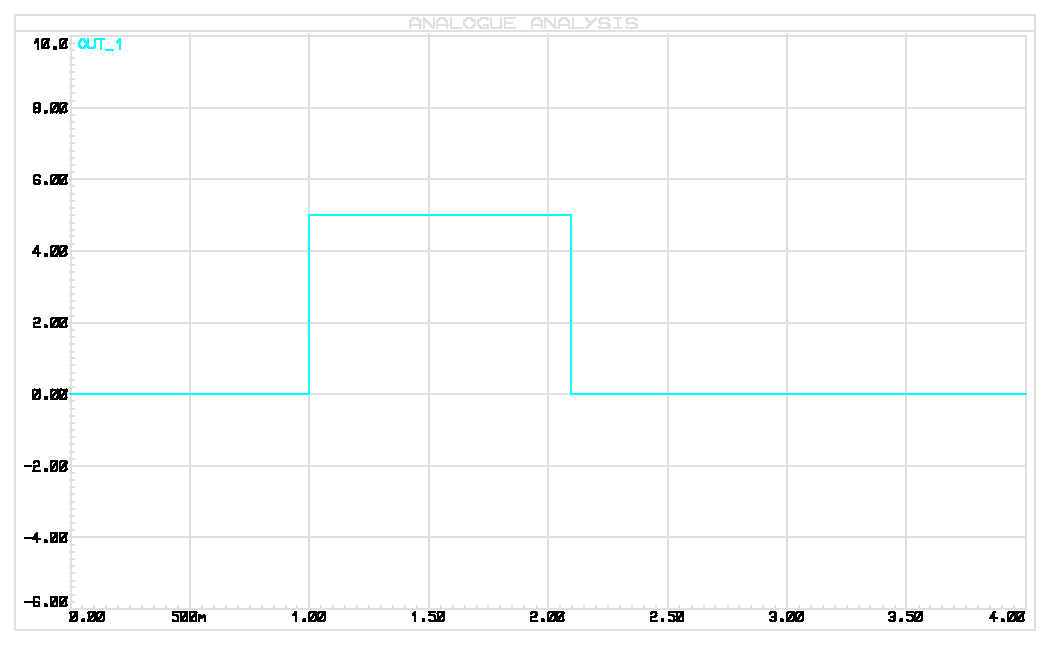
\includegraphics[scale=0.75]{Graphics/Practice 2/GRAPHICS/ANIMATION/555/555_MONO_ANALOGUE_F1.PDF}
    }\fi
    
    \caption{Analog Analysis of a Monostable Multivibrator.}
    \label{fig:555_MONO_ASSEMBLY}
\end{figure}

\clearpage


\section{Laboratory Lecture 3: Stepper Motor Controller}

\subsection{Introduction}

The aim of this practice is to go over the basics of how to control a stepper motor. A stepper motor is a brushless DC electric motor that divides a full rotation in several small increments or \textit{steps}. By providing power to its coils in a specific way, we can control the position of the shaft.\medskip

Stepper motors can be unipolar or bipolar. Unipolar Stepper motors are very similar to Bipolar Stepper Motors, but are manufactured with a central tap that connects back to the power source, essentially splitting each coil into two smaller coils that can be powered independently. If required, the central tap can also be left disconnected, allowing the Unipolar Stepper Motor to be converted into a Bipolar configuration.\medskip

Bipolar Stepper Motors do not feature a central tap for dividing their solenoid coils. This makes their internal wiring slightly less complex than that of a Unipolar Motor.

\vspace{0.3cm}

\begin{figure}[H]
    \centering
    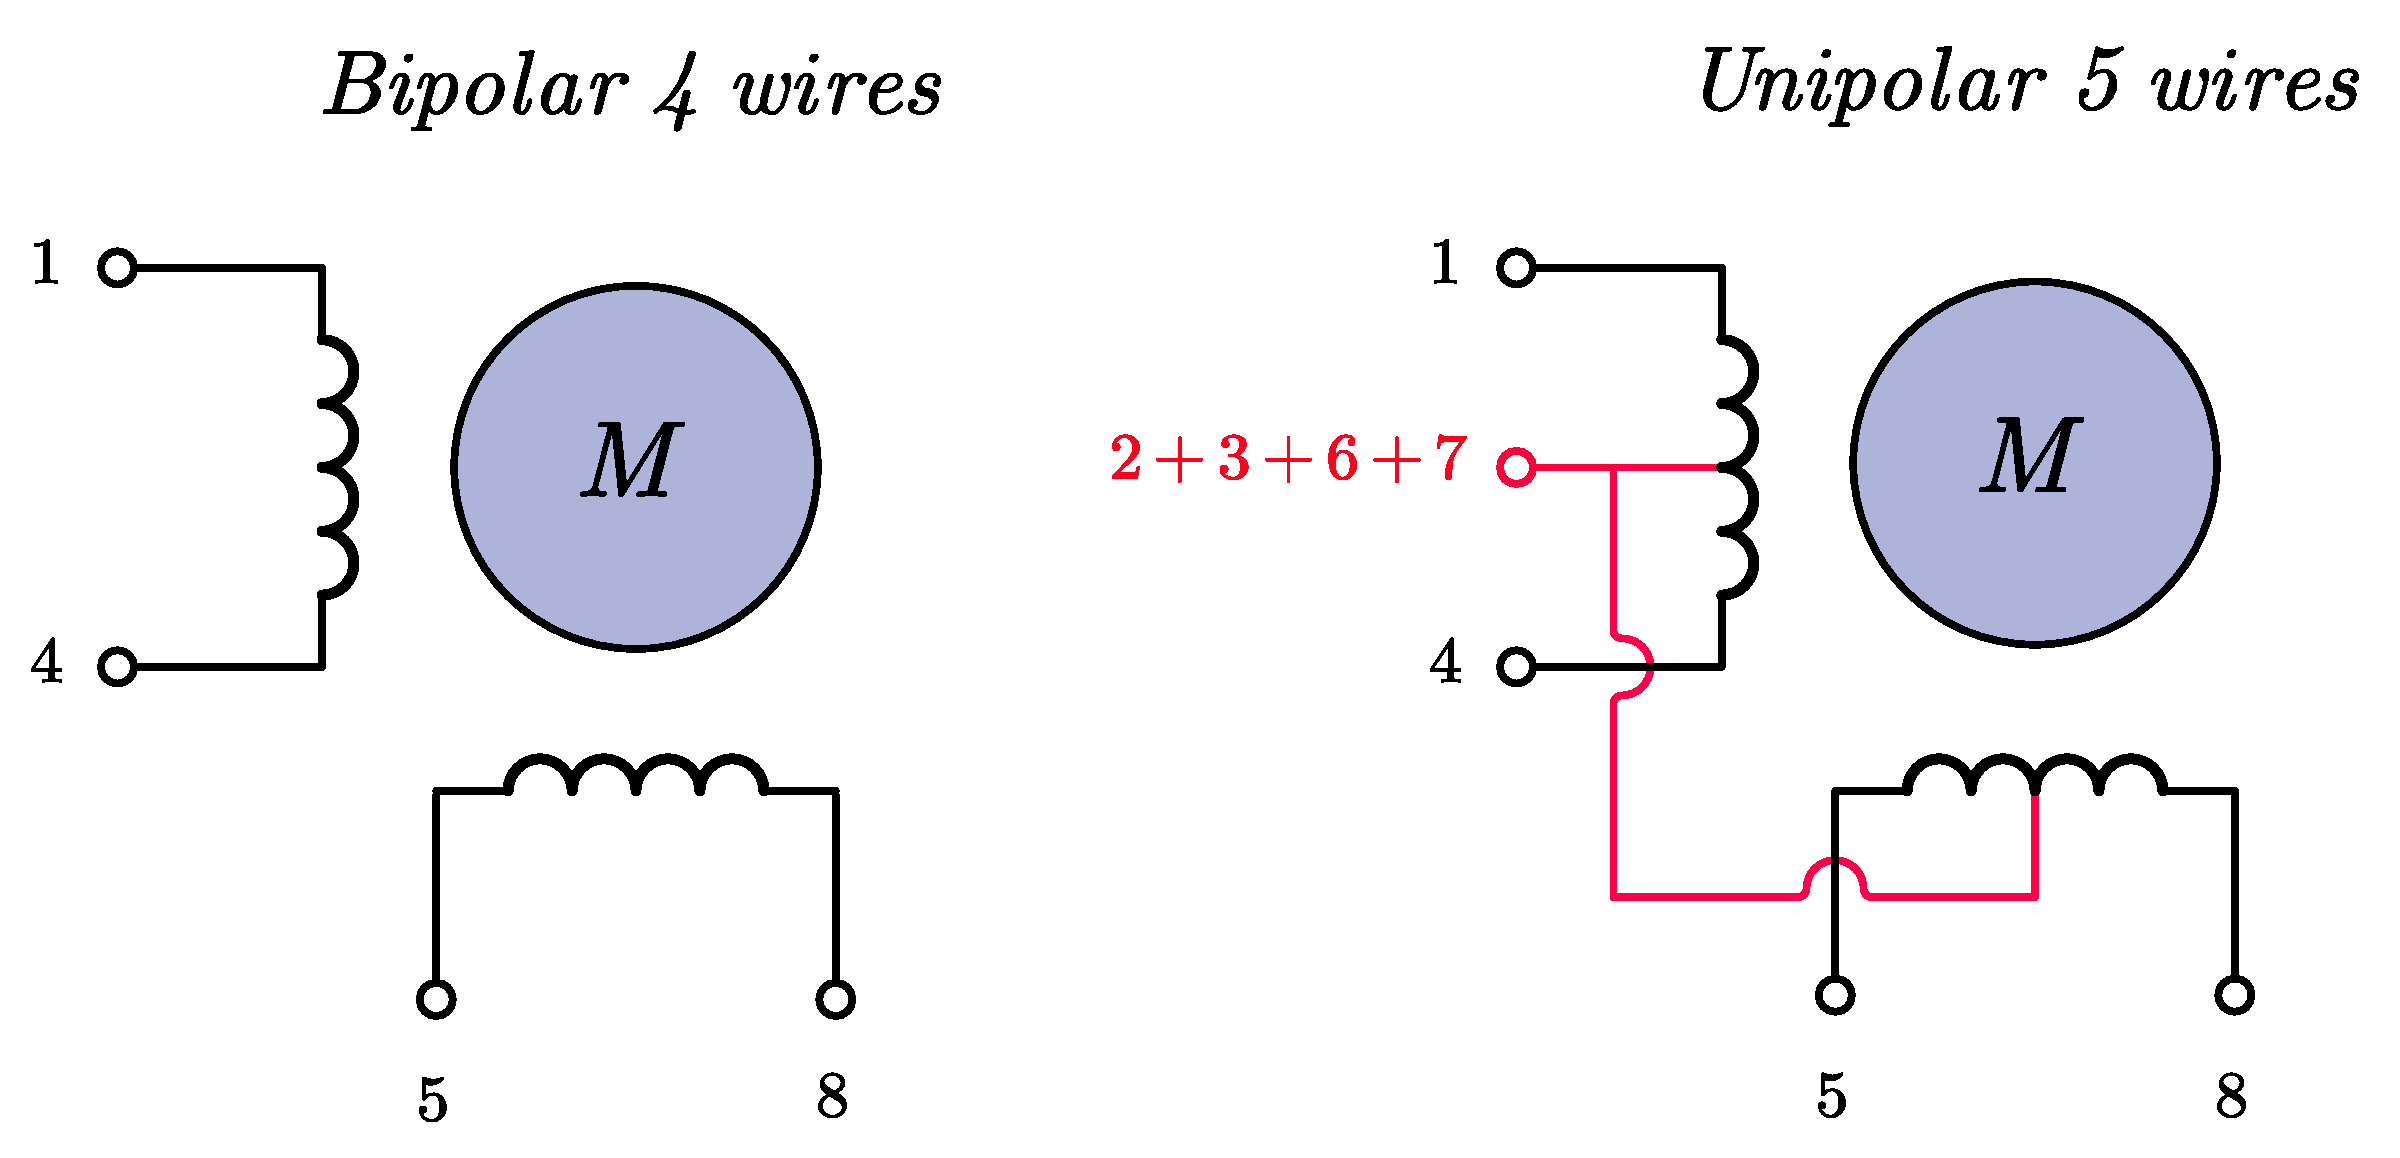
\includegraphics[scale = 0.24]{Graphics/Practice 3/GRAPHICS/STEPPER_TYPES.pdf}
    \caption{Bipolar vs. Unipolar configurations.}
    \label{fig:STEPPER_TYPE}
\end{figure}

\clearpage

\subsection{Stepper Motor Controller}

In this practice we will use the Bipolar type, in particular a NEMA 17 motor. To control it we will use a special driver, the L293D, which is basically an array or darlington transistors, in half-H configuration,  whose main objective is to take care of switching the high currents that the motors require. 

\vspace{0.3cm}

\begin{figure}[H]
    \centering
    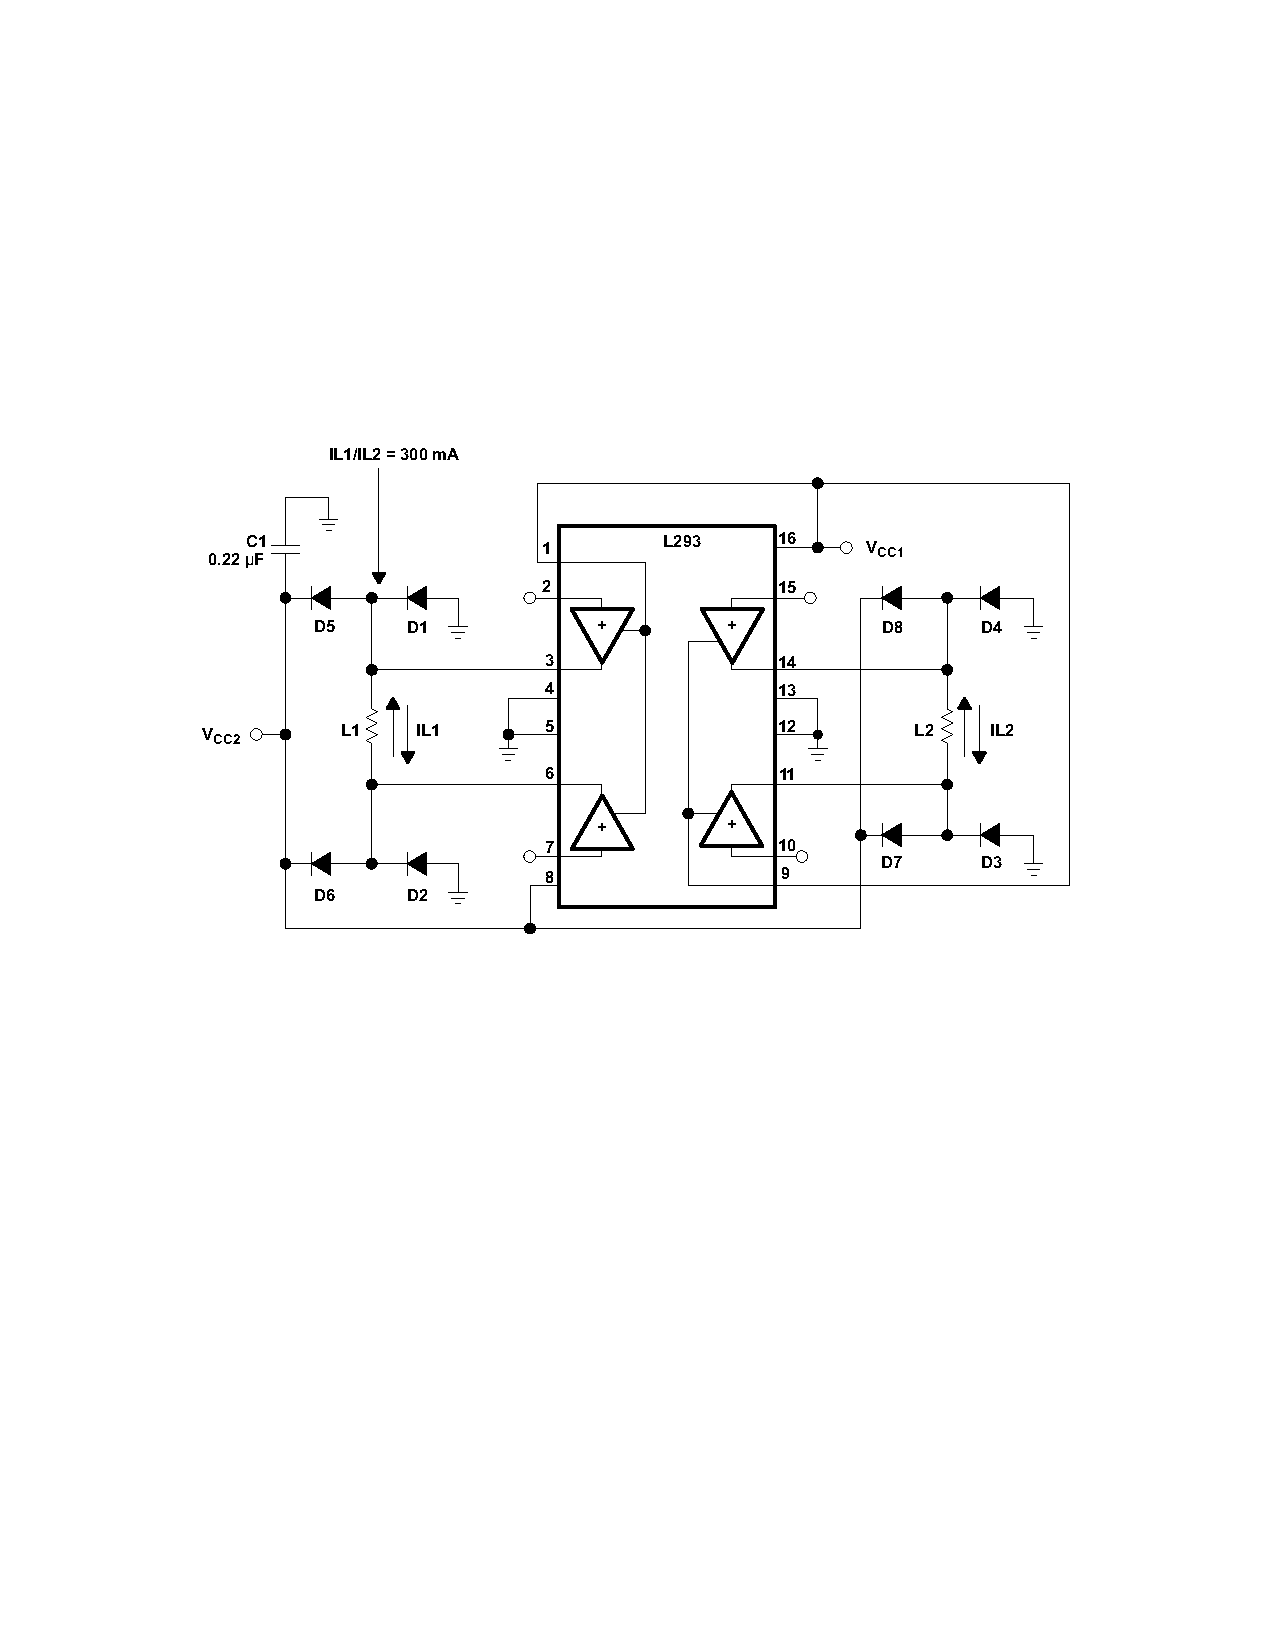
\includegraphics[scale = 0.85]{Graphics/Practice 3/GRAPHICS/DATASHEETS/L293D_INTERNAL.pdf}
    \caption{L293D Bipolar Stepper Controller. ~\autocite{L293D}}
    \label{fig:L293D}
\end{figure}

To control said driver, we will make us of the SPLD that we have been using since the beginning, the GAL22V10C and some basic VHDL code. In order to make the shaft spin in a controlled manner, we have to take into account the phase current waveforms, i.e. the pulses that we have to send to the driver to cause a step change and the order in which they must be sent. This information can be seen below:

\vspace{0.3cm}

\begin{table}[ht]
    \centering
        \begin{tabular}[t]{lcccc}
            \toprule
            &\textbf{Step}&\textbf{Full-Step [1.8\textdegree]}&\textbf{Wave-Step [1.8\textdegree]}&\textbf{Half-Step [0.9\textdegree]}\\
            \midrule
            & 0 & 1010 & 1000 & 1010\\
            & 1 & 1001 & 0001 & 1000\\
            & 2 & 0101 & 0100 & 1001\\
            & 3 & 0110 & 0010 & 0001\\
            & 4 &      &      & 0101\\
            & 5 &      &      & 0100\\
            & 6 &      &      & 0110\\
            & 7 &      &      & 0010\\
            \bottomrule
        \end{tabular}
        \caption{Phase Current Waveforms. ~\autocite{SLIDES_3}}
        \label{table: PHASE_CURRENT_WAVEFORMS}
\end{table}

\subsubsection{VHDL Code}

As we have seen in Table \ref{table: PHASE_CURRENT_WAVEFORMS}, there are 3 different ways in which we can control the rotation of the stepper motor, namely, full-step, wave-step and half-step. Each of them present advantages and disadvantages. For instance, \textit{Half-Steps} can deliver a higher precision, since every step only spins the shaft 0.9\textdegree as opposed to \textit{full-step} and \textit{wave-step}, which spin it 1.8\textdegree. This increase in performance reduces the output torque significantly, so there is a clear trade-off between both variables that one must consider. In addition to this, \textit{Wave-step} mode is more visually appealing, as the transitions between states are not as choppy as with the other ones.\medskip

Due to the limitations that the GAL22V10C possesses, it is not possible to fit the 3 control modes in the same SPLD. That's why we have developed 3 different codes, one for each, that can be seen below:

\paragraph{Full Step}

\begin{code}{vhdl}
library ieee;
use ieee.std_logic_1164.all;

entity STEPPER_FS is
  port(CLK: in std_logic;
       DIR: in std_logic;
       MOTOR: out std_logic_vector(3 downto 0)
       );
end STEPPER_FS;

architecture ARCH of STEPPER_FS is
  begin
    process(CLK)
      variable COUNT: std_logic_vector(3 downto 0);
        begin
          if(CLK'EVENT and CLK='1') then

            if(DIR='0') then
              case COUNT is
                when "0000" => COUNT := "1010";
                when "1010" => COUNT := "1001";
                when "1001" => COUNT := "0101";
                when "0101" => COUNT := "0110";
                when "0110" => COUNT := "1010";
                when others => COUNT := "0000";
              end case;
              
              
              
                else
                  case COUNT is
                    when "0000" => COUNT := "0110";
                    when "0110" => COUNT := "0101";
                    when "0101" => COUNT := "1001";
                    when "1001" => COUNT := "1010";
                    when "1010" => COUNT := "0110";
                    when others => COUNT := "0000";
                  end case;
            end if;
          end if;
        
          MOTOR <= COUNT;
          
    end process;
end ARCH;
\end{code}

As we have previously mentioned, \textit{Full Step} phase control provides the highest torque of all, though the transitions tend to look quite choppy. This mode and the \textit{Wave Step} one provide a maximum accuracy of 1.8\textdegree \, per step, which means that a full 360\textdegree \, rotation would require 200 steps.\medskip

The code that we have included moves the shaft one step (forwards or backwards) whenever a \textit{PGT} occurs. This indicates that the process is synchronous. Besides, we can also find a direction pin which changes the direction of the spin when a positive signal is applied to it.

\paragraph{Wave Step}

\begin{code}{vhdl}
library ieee;
use ieee.std_logic_1164.all;

entity STEPPER_WS is
  port(CLK: in std_logic;
       DIR: in std_logic;
       MOTOR: out std_logic_vector(3 downto 0)
       );
end STEPPER_WS;

architecture ARCH of STEPPER_WS is
  begin
    process(CLK)
      variable COUNT: std_logic_vector(3 downto 0);
        begin
          if(CLK'EVENT and CLK='1') then

            if(DIR='0') then
              case COUNT is
                when "0000" => COUNT := "1000";
                when "1000" => COUNT := "0001";
                when "0001" => COUNT := "0100";
                when "0100" => COUNT := "0010";
                when "0010" => COUNT := "1000";
                when others => COUNT := "0000";
              end case;
              
                else
                  case COUNT is
                    when "0000" => COUNT := "0010";
                    when "0010" => COUNT := "0100";
                    when "0100" => COUNT := "0001";
                    when "0001" => COUNT := "1000";
                    when "1000" => COUNT := "0010";
                    when others => COUNT := "0000";
                  end case;
            end if;
          end if;
        
          MOTOR <= COUNT;
          
    end process;
end ARCH;
\end{code}

This code describes the \textit{Wave Step} phase control sequence. Wave Stepping is usually used when the smoothness of the output rotation is important. As per the last mode, this mode has a high torque but its trade-off is a reduction in its accuracy. \medskip

The rest of the code remains the same as the last one.

\paragraph{Half Step}

\begin{code}{vhdl}
library ieee;
use ieee.std_logic_1164.all;

entity STEPPER_HS is
  port(CLK: in std_logic;
       DIR: in std_logic;
       MOTOR: out std_logic_vector(3 downto 0)
       );
end STEPPER_HS;

architecture ARCH of STEPPER_HS is
  begin
    process(CLK)
      variable COUNT: std_logic_vector(3 downto 0);
        begin
          if(CLK'EVENT and CLK='1') then

            if(DIR='0') then
              case COUNT is
                when "0000" => COUNT := "1010";
                when "1010" => COUNT := "1000";
                when "1000" => COUNT := "1001";
                when "1001" => COUNT := "0001";
                when "0001" => COUNT := "0101";
                when "0101" => COUNT := "0100";
                when "0100" => COUNT := "0110";
                when "0110" => COUNT := "0010";
                when "0010" => COUNT := "1010";
                when others => COUNT := "0000";                            
            end case;
              
                else
                  case COUNT is
                    when "0000" => COUNT := "0010";
                    when "0010" => COUNT := "0110";
                    when "0110" => COUNT := "0100";
                    when "0100" => COUNT := "0101";
                    when "0101" => COUNT := "0001";
                    when "0001" => COUNT := "1001";
                    when "1001" => COUNT := "1000";
                    when "1000" => COUNT := "1010";
                    when "1010" => COUNT := "0010";
                    when others => COUNT := "0000";
                  end case;
            end if;
          end if;
        
          MOTOR <= COUNT;
          
    end process;
end ARCH;
\end{code}

In addition, we can find the \textit{Half Step} phase control sequence. As we can see, this code is longer than the last 2 codes. This is due to the fact that it has some intermediate states which help smooth out the rotation by getting rid of most of the chopping that characterizes the latter.


\subsubsection{Proteus Simulation and Assembly}

After discussing the code, we will move on to the simulation of the circuit. For this we will use ISIS Proteus once again. Even though Figure \ref{fig:L293D} may look cumbersome, in actuality, we only have to connect the 2 coils to the driver's output and the 4 direction pins to its inputs following this fashion:\medskip

\begin{figure}[H]
    \centering
    
    \ifnum\value{ANIMATION}=1 {
        \animategraphics[controls,loop,scale=0.8]{1}{Graphics/Practice 3/GRAPHICS/ANIMATION/F}{0}{8}
    } 
    \else {
        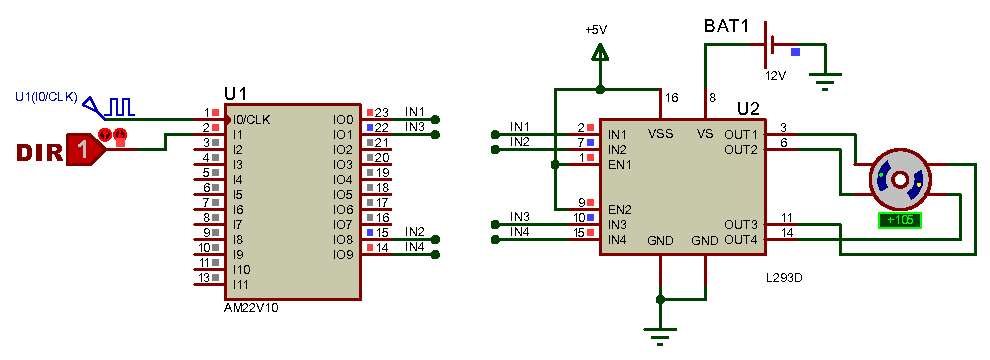
\includegraphics[scale=0.8]{Graphics/Practice 3/GRAPHICS/ANIMATION/F5.PDF}
    }\fi
    
    \caption{Stepper with rotation direction control.}
    \label{fig:STEPPER_ROTATION}
\end{figure}

The I/O pins that we used are the ones that the the compiler assigned by default. They are displayed in the Chip Report (Figure \ref{fig:CHIP_REPORT}).\medskip

Assembling the circuit is just a matter of manually connecting everything following the schematic of Figure \ref{fig:STEPPER_ROTATION}. To provide a clock signal we have used a signal generator which output has been set to a TTL level, 0 to 5V, and its frequency to 1 Hz.  

\clearpage

\section{Laboratory Lecture 3: Stepper Motor Controller}

This is my last test



\clearpage
\printbibliography


\end{document}